\documentclass[10pt,spanish,a4paper,openany,notitlepage]{article}
\usepackage[spanish,es-tabla]{babel}  	% Traduce los textos a castellano
\usepackage[utf8]{inputenc}
\usepackage{units}
\usepackage{fancyhdr}
\usepackage{anysize}
\usepackage{float}
\usepackage[dvipsnames]{xcolor}
\usepackage{abstract} % paquete para el resumen del articulo
\usepackage{natbib}
\usepackage{graphicx}
\usepackage{tablefootnote} % para agregar notas al pie de pagina en las tablas
\usepackage{amsmath} % para agregar acentos a las variables matematicas, como por ej ^ para indicar el valor pico
\usepackage{hyperref} % para agregar url
\usepackage[bottom]{footmisc} % para que las footnote esten al final de la hoja y no cuando termina el texto
\usepackage{multirow}

\setcitestyle{square} %cambio las citas a [] en lugar de ()

% todo lo que sigue es para poner links que se les pueda hacer click
\usepackage{xcolor}
\usepackage[normalem]{ulem}
\usepackage{hyperref}
\hypersetup{colorlinks,urlcolor=blue}

\makeatletter
\DeclareUrlCommand\ULurl@@{%
  \def\UrlFont{\ttfamily\color{blue}}%
  \def\UrlLeft{\uline\bgroup}%
  \def\UrlRight{\egroup}}
\def\ULurl@#1{\hyper@linkurl{\ULurl@@{#1}}{#1}}
\DeclareRobustCommand*\ULurl{\hyper@normalise\ULurl@}
\makeatother

%---------------------------------------Configuraciones de pagina----------------------------------------------
\marginsize{2.5cm}{2.5cm}{1cm}{1cm}

\pagestyle{fancy}
\fancyhf{}
\lhead{
86.06 - \textsc{Circuitos Electrónicos}\\ 
1\textsuperscript{er} Cuatrimestre de 2016
}
\rhead{
\includegraphics[width=3cm]{includes/FIUBA_ALTA.jpg}}
\rfoot{Página \thepage}

%------------------------------ graphicx ----------------------------------
%
% Todas las im�genes est�n en el directorio tp-img:
%
\newcommand{\imgdir}{includes}
\graphicspath{{\imgdir/}}
%


%------------------------- Inicio del documento ---------------------------

\begin{document}

\begin{titlepage}

\thispagestyle{empty}

\begin{center}

\includegraphics[scale=0.3]{fiuba}\\
\large{\textsc{Universidad de Buenos Aires}}\\
\large{\textsc{Facultad De Ingeniera}}\\
\small{2016 - 1\textsuperscript{er} Cuatrimestre}
\end{center}

\vfill

\begin{center}
\Large{\underline{86.06 - \textsc{Circuitos Electrónicos}}}
\end{center}

\vfill

\begin{tabbing}
\hspace{2cm}\=\+TRABAJO DE LABORATORIO 1\\
	Amplificadores Operacionales: Usos y Limitaciones\\
	\today\\
\\
	INTEGRANTES:\hspace{-1cm}\=\+\hspace{1cm}\=\hspace{6cm}\=\\
		Bruno, Nicolas	\>\> 95191\\
			\>\footnotesize{$<$nicoo.24@hotmail.com$>$}\\
		Hagata, Juan Pablo	\>\> 93856\\
			\>\footnotesize{$<$jpablo.hagata@gmail.com$>$}\\
		Vazquez, Matias	\>\> 91523\\
			\>\footnotesize{$<$mfvazquezfiuba@gmail.com$>$}\\
\end{tabbing}

\vfill

\hrule
\vspace{0.2cm}

\end{titlepage}

%
% Hago que las pginas se comiencen a contar a partir de aqu�
%
\setcounter{page}{1}

%
% Pongo el �ndice en una p�gina aparte:
%
\tableofcontents
\newpage


\section{Introducción}

En el siguiente trabajo se presentará a través de mediciones en laboratorio, la utilización
de circuitos integrados analógicos y componentes asociados para la realización de distintas funciones.
Se observarán las limitaciones que presenta el uso de los modelos representativos del funcionamiento de
dichos circuitos integrados para predecir su comportamiento, como así también la influencia de las
características del instrumental utilizado en la medición, en los valores obtenidos.

Los CI analógicos llamados Amplificadores Operacionales – AO – presentan una versatilidad
tal que permiten, además de amplificar tensión, realizar circuitalmente la mayoría de operaciones matemáticas
lineales y no lineales sobre señales analógicas, como ser: multiplicación de una señal por una
constante (equivalente a amplificar linealmente con el mismo valor de amplificación a todas las componentes
significativas de su espectro de frecuencias), suma algebraica de señales, producto de señales
(que incluye obtener la señal elevada a un exponente), derivación e integración de señales u obtener el
logaritmo o la exponencial de una señal. Para realizar estas funciones deberán conectarse en forma
conveniente a los terminales de los AO, componentes exteriores – resistores, capacitores, diodos, transistores,
etc -.

El AOV más simple posee tres terminales para tensión de señal y dos para conectar las tensiones
continuas de alimentación para polarizar los transistores que conforman el CI.

De los tres terminales de señal, dos son de entrada o excitación y uno de salida. Las señales
aplicadas a los dos terminales de entrada y la señal en el terminal de salida sobre la carga, están referidas
a un punto o línea del circuito completo (el CI con los componentes externos asociados), que
puede o no tener conexión directa con algún terminal del CI, que será lo que normalmente se conoce
como terminal común, línea de común o masa del circuito.

Los otros dos terminales sirven para la conexión de una o dos fuentes de tensión continua de
alimentación. De utilizarse una, positiva o negativa, el otro terminal de fuente de alimentación del CI
irá conectado al punto común del circuito completo, y de utilizarse dos, una positiva y la otra negativa,
el terminal opuesto de cada fuente de tensión continua de alimentación irá conectado a ese punto
común, como puede verse en la figura \ref{fig:AO}

\begin{figure}[H]
\centering
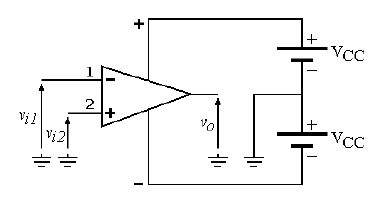
\includegraphics[scale=1]{circuitos/AO.png}
\caption{Amplificador Operacional}
\label{fig:AO}
\end{figure}

La utilización de dos fuentes de tensión continua de alimentación de distinto signo, permite que
la tensión de polarización del terminal de salida respecto a común - $V_{OQ}$ – pueda ser nula. Este tipo de
alimentación se conoce como de \textquotedblleft fuente partida\textquotedblright o \textquotedblleft fuente simétrica\textquotedblright en el caso de ser de igual valor.
La tensión en el terminal de salida de los amplificadores conocidos como AOV – $V_o$ -, es función
de la diferencia de la señal de tensión de las dos entradas. A esta diferencia de las dos señales de entrada
las denominaremos señal de excitación o entrada diferencial y la distinguiremos con el subíndice
\textquotedblleft d\textquotedblright – $v_{id}$ -. Si el AOV trabaja como amplificador lineal con valores de señales suficientemente
pequeños como para admitir esta aproximación dentro de las tolerancias requeridas, $V_o$ será proporcional
a $v_{id}$ resultando:

\begin{equation}
    V_o = A_{vd0} (V_{i1} - V_{i2}) = A_{vd0} V_{id}
    \label{eq:V_o}
\end{equation}


Donde $V_o$ es la tensión entre el terminal de salida y común,
$V_{id} = (V_{i1} - V_{i2})$ es la diferencia entre las
señales aplicadas a los terminales de entrada referidas a común y la constante de proporcionalidad $A_{vd0}$
es la amplificación de tensión con entrada diferencial o simplemente amplificación de tensión del AOV,
que podrá ser un número complejo o real según existan o no efectos reactivos en el CI. El subíndice
\textquotedblleft 0\textquotedblright de $A_{vd0}$ indica que se ha supuesto que no hay ningún componente adicional conectado a los terminales
del AOV, a excepción de los dos generadores de tensión de señal de excitación (considerados
generadores ideales), la o las dos fuentes de alimentación de continua para polarizarlo y que el amplificador
procesa la señal con su terminal de salida en vacío – $R_L \rightarrow \infty$ -. De la expresión \ref{eq:V_o} surge que
$A_{vd0}$ se definirá como:

\begin{equation}
    A_{vd0} = \frac{V_o}{V_{id}} \Biggr|_{I_o = 0}
    \label{eq:A_vd0}
\end{equation}

Si se aplica una señal senoidal $V_{i1}$ al terminal 1 de entrada indicado, con el terminal 2 conectado a
común, se tiene una señal de salida $V_o$ opuesta en fase a $v_{i1}$ (signo – en el terminal 1 de entrada), en
tanto que al aplicar la señal en el 2, $V_{i2}$, con el terminal 1 a común, la señal de salida $V_o$ estará en
fase con $V_{i2}$ (signo + en el terminal 2 de entrada). Por este motivo se denomina terminal de entrada
inversor al terminal denominado 1 en la figura, indicado con el signo - y terminal de entrada
no inversor al terminal denominado 2 en la figura, indicado con el signo +.

Los AOV se utilizan siempre con alguna conexión (directa o a través de algún componente) entre
su terminal de salida y uno o ambos terminales de entrada, lo que significa que existirá una realimentación
entre la salida y la entrada del amplificador. En circuitos amplificadores esta realimentación
será normalmente de tipo negativa, es decir, desde la salida se introducirá en la entrada una tensión o
corriente de señal que se restará de la señal aplicada en la entrada y la diferencia entre ambas será
procesada por el circuito. Cuando existe realimentación y por ende alguna conexión desde la salida a la
entrada de un amplificador, significa que está trabajando con un lazo cerrado de realimentación y por
contraposición, si no existe ninguna realimentación se dice que el amplificador trabaja a lazo abierto.

Por esta última razón, la amplificación de un AOV, tal como se muestra en la figura \ref{fig:AO}, sin ningún
otro componente asociado que los que se muestran, será una amplificación a lazo abierto y en
vacío, ya que la no existencia de ninguna impedancia de carga conectada al terminal de salida, implica
que esta sea infinita. La amplificación de tensión definida en \ref{eq:A_vd0} se podrá indicar en este caso como:

\begin{equation}
    A_{vd0} = A_{vdol} = A_{vol} = \frac{V_o}{V_{id}} = \frac{V_o}{V_i}
    \label{eq:A_vol}
\end{equation}

Donde el subíndice \textquotedblleft ol\textquotedblright significa lazo abierto y la  \textquotedblleft d\textquotedblright se ha eliminado en $A_v$ y en $V_i$ pues la amplificación
de tensión a lazo abierto de un AOV se define directamente para entrada diferencial y con el
AOV trabajando en vacío, por lo que tampoco se ha indicado que la relación entre las tensiones se obtiene
con la condición $i_o = 0$.

Para el análisis del funcionamiento de un circuito con un AOV y componentes asociados, incluyendo
la impedancia de carga, puede suponerse con suficiente aproximación en numerosas aplicaciones,
que el AO se comporta como un AOV ideal.

El AOV ideal se define como un amplificador que posee las siguientes propiedades:

\begin{equation}
    A_{vol} \rightarrow \infty
    \label{eq:Avol_ideal}
\end{equation}

\begin{equation}
    R_i \rightarrow \infty
    \label{eq:Ri_ideal}
\end{equation}

\begin{equation}
    R_o = 0
    \label{eq:Ro_ideal}
\end{equation}

\begin{equation}
    \text{Ancho de banda AB} \rightarrow \infty
    \label{eq:ABbanda_ideal}
\end{equation}

La condición \ref{eq:ABbanda_ideal} implica que se admite que el AO no posee efectos reactivos y por lo tanto el
valor de $A_{vol}$ se mantiene para frecuencias de onda senoidal comprendidas entre $f = 0$ y $f \rightarrow \infty $, y las
impedancias de entrada y salida son resistivas puras. $R_i$ es la resistencia de Thevenin \textquotedblleft vista\textquotedblright entre
ambos terminales de entrada del AO y $R_o$ la resistencia de Thevenin \textquotedblleft vista\textquotedblright entre el terminal de salida
del AO \textquotedblleft mirando\textquotedblright hacia éste.

A continuación se enunciaran configuraciones del AO utilizadas en el trabajo, con sus respectivas ecuaciones.

\subsection{Amplificador de tensión o multiplicador por una constante}

Se muestra en la figura \ref{fig:intro_amplificador} el circuito de señal, sin reemplazar el AO por su modelo.

\begin{figure}[H]
\centering
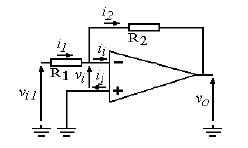
\includegraphics[scale=1]{circuitos/amplificador.png}
\caption{Circuito amplificador}
\label{fig:intro_amplificador}
\end{figure}

Utilizando las propiedades de AOV ideal se llega a las siguientes ecuaciones:

\[ \displaystyle i_1 = \frac{(V_{i1} - V_i)}{R_1} = \frac{V_{i1}}{R_1} \]

\[ \displaystyle i_2 = \frac{(V_i - V_o)}{R_2} = -\frac{V_o}{R_2} \]

Dado que $i_i = 0$, debido a la propiedad \ref{eq:Ri_ideal}, resulta $i_1 = i_2$

Igualando las ecuaciones se obtiene:

\[ \displaystyle \frac{V_{i1}}{R_1} = -\frac{V_o}{R_2} \]

La amplificación de tensión entre el terminal de salida $V_o$ y la tensión aplicada proveniente del
generador de excitación $V_{i1}$ será una amplificación de tensión a lazo cerrado o amplificación de
tensión del circuito realimentado, que se define como:

\[ \displaystyle A_v = \frac{V_o}{V_{i1}} \]

Resultando:

\begin{equation}
    A_v = \frac{V_o}{V_{i1}} = -\frac{R_2}{R_1}
\label{eq:gan_amplificador}
\end{equation}

Finalmente se obtiene la $V_o$ en función de $V_{i1}$.

\begin{equation}
    V_o = A_v V_{i1}
    \label{eq:amplificador}
\end{equation}


\subsection{Circuito integrador}

Se muestra en la figura \ref{fig:intro_integrador} el circuito de señal, sin reemplazar el AO por su modelo.


\begin{figure}[H]
\centering
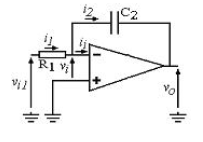
\includegraphics[scale=1]{circuitos/integrador.png}
\caption{Circuito integrador}
\label{fig:intro_integrador}
\end{figure}

Dado que $v_i = 0$ ya que $i_i = 0$ resulta:

\[ \displaystyle i_1 = \frac{V_{i1}}{R_1} \]

\[ \displaystyle i_2 = -C_2 \frac{dV_o}{dt} \]

Como $i_1 = i_2$ se tiene:

\[ \displaystyle \frac{V_{i1}}{R_1} = -C_2 \frac{dV_o}{dt} \]

Finalmente se obtiene:

\begin{equation}
    v_o = \frac{-1}{R_1 C_2} \int v_{i1} dt = \frac{-1}{\tau} \int v_{i1} dt
    \label{eq:integrador}
\end{equation}

\section{Trabajo de Laboratorio}

Se utilizará un AO LM741 alimentado con dos fuentes simétricas de $\pm 12\, \unit{V}$

A solo efecto de poner en evidencia los valores que limitan el funcionamiento del AO LM741 utilizado, 
se resumen las siguientes características básicas de su funcionamiento.

\begin{table}[H]
\centering
\begin{tabular}{|c|c|}
\hline
$R_I$ & $2 \,\unit{M\Omega} $  \\ \hline
$R_O$ & $75 \,\unit{\Omega} $ \\ \hline
$A_{vol}$ & $200000$ \\ \hline
$I_{bias}$ & $80 \,\unit{nA} $ \\ \hline
$I_{os}$\tablefootnote{corriente de salida en cortocircuito} & $25 \,\unit{mA} $ \\ \hline
$V_{off}$ & $2 \,\unit{mV} $ \\ \hline
$I_{off}$ & $10 \,\unit{nA} $ \\ \hline
\end{tabular}
\caption{Características básicas del AO LM741}
\label{table:caracteristicas_LM741}
\end{table}

\section{Amplificador de tensión o multiplicador por una constante}

Se utilizará el banco de medición mostrado en la figura \ref{fig:amplificador} con distintas configuraciones.

\begin{figure}[H]
\centering
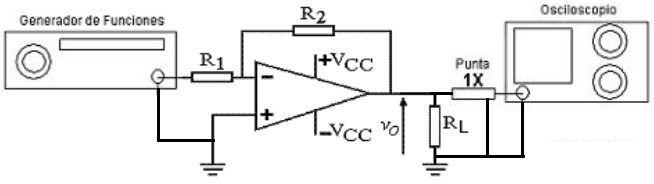
\includegraphics[scale=0.8]{circuitos/A1.png}
\caption{Banco de medición del circuito amplificador}
\label{fig:amplificador}
\end{figure}

Se calcula la tensión de salida del circuito mediante la ecuación \ref{eq:amplificador}. Para calcular ganancia se utilizará la ecuación \ref{eq:gan_amplificador}.

\begin{enumerate}
\item Obtener el valor de la tensión pico de salida del circuito y su forma de 
de variación temporal para una entrada senoidal de $1\,\unit{KHz}$ y $\overset{\wedge}{V}_{i1} = 0.2\,\unit{V}$
, con $R_L = 1\,\unit{K\Omega}$ y los siguientes valores de $R_1$ y $R_2$

\begin{enumerate}
    \item $R_1 = 1\,\unit{K\Omega}$ $R_2 = 10\,\unit{K\Omega}$
    
    Mediante las ecuaciones \ref{eq:amplificador} y \ref{eq:gan_amplificador}  se obtiene $\overset{\wedge}{V}_o = 2\,\unit{V}$ y $A_v$=-10
    
    Simulando en \emph{Spice} se obtiene la señal de salida mostrada en la
    figura \ref{fig:vo_1a}. Para realizar la simulación en  \emph{Spice} se agrego
    también (a la entrada y a la salida) el modelo equivalente de la punta x1.
    
    \begin{figure}[H]
    \centering
    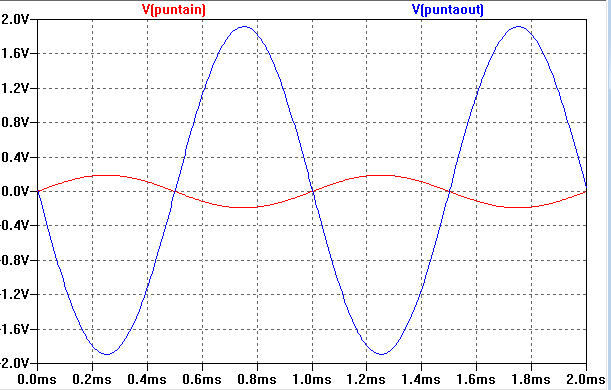
\includegraphics[scale=0.8]{simulaciones/A1A.png}
    \caption{Simulación de la tensión de salida}
    \label{fig:vo_1a}
    \end{figure}
    
    \begin{figure}[H]
    \centering
    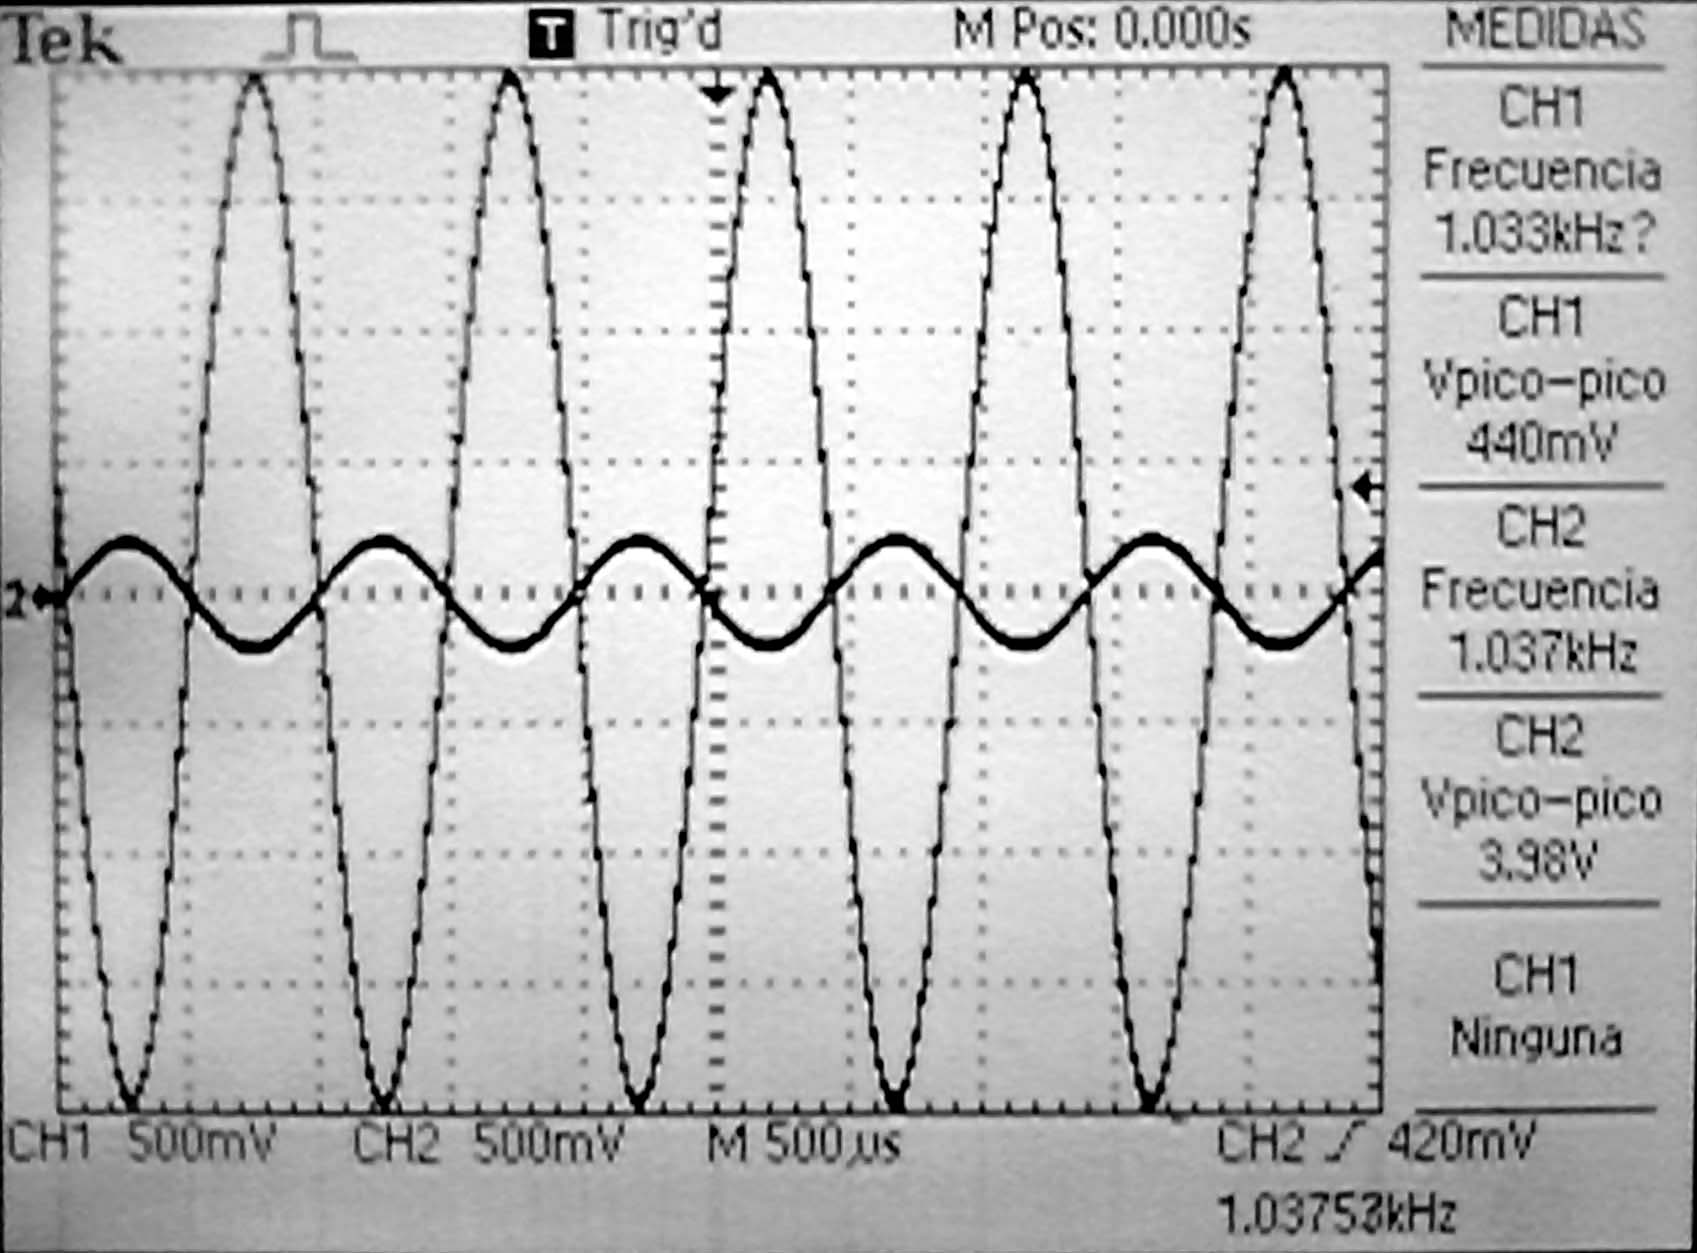
\includegraphics[width=350pt, height=250pt]{mediciones/A1a.jpg}
    \caption{Medición de la tensión de salida}
    \label{fig:vo_med_1a}
    \end{figure}
    
    De las figuras \ref{fig:vo_1a} y \ref{fig:vo_med_1a} puede observarse que no hay diferencias
    perceptibles entre lo simulado y lo medido, ya que el valor pico de la medición fue de $1.99\,\unit{V}$ y el de la simulación $1.90\,\unit{V}$, que son valores muy próximo al ideal, $2\,\unit{V}$ . Respecto a la ganancia, la medida resultó de $-9.04$ y la simulada de $-9.5$ que están alejados del valor ideal calculado al principio que fue de $-10$.\\
    
    
    Luego se reemplazó $R_L$ por $R_L = 10\,\unit{\Omega}$. Del modelo se espera observar lo mismo que en el inciso a) ya que no se modifican los valores de resistencias que determinan la ganancia y por lo tanto, el valor de salida. Simulando en \emph{Spice} se obtiene la señal de salida mostrada en la figura \ref{fig:vo_1aRL}.
 
    
    \begin{figure}[H]
    \centering
    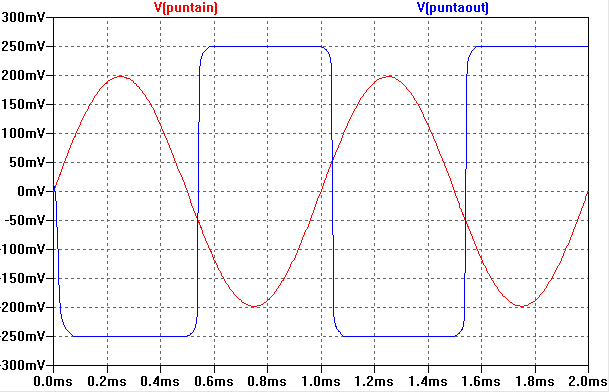
\includegraphics[scale=0.8]{simulaciones/A1A-Rl10ohm.png}
    \caption{Simulación de la tensión de salida con $R_L = 10\,\unit{\Omega}$}
    \label{fig:vo_1aRL}
    \end{figure}
    
    \begin{figure}[H]
    \centering
    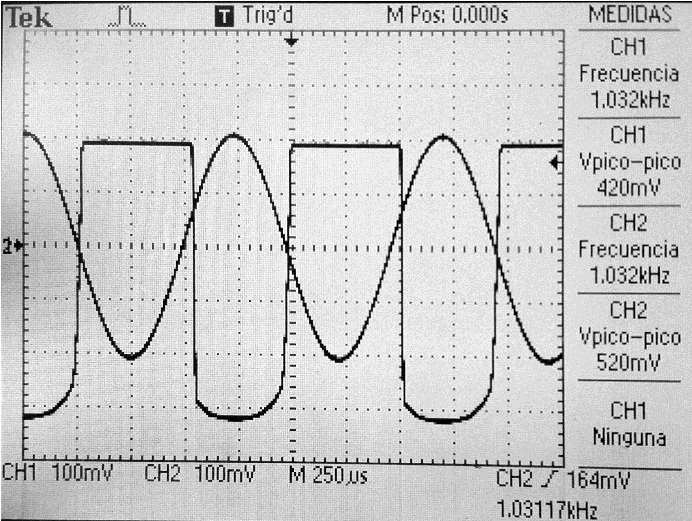
\includegraphics[width=350pt, height=250pt]{mediciones/A1a-10R-ultima_preg.jpg}
    \caption{Medición de la tensión de salida con $R_L = 10\,\unit{\Omega}$}
    \label{fig:vo_med_1aRL}
    \end{figure}
    
    
    De las figuras \ref{fig:vo_1aRL} y \ref{fig:vo_med_1aRL} puede observarse una cierta diferencia. En la medición el CH1 corresponde a la señal de entrada, y CH2 a la señal de salida. En este caso la tensión de entrada es de $220\unit{mV}$ pico en lugar de $200\unit{mV}$ y la salida de $260\unit{mV}$ pico en lugar de $250\unit{mV}$ pico. La parte positiva tiene un valor pico de $200\unit{mV}$ y la parte negativa de $300\unit{mV}$ ya que los AO, constructivamente, poseen limitaciones para los valores máximos de uno u otro semiciclo. \\
    
    \item $R_1 = 1\,\unit{M\Omega}$ $R_2 = 10\,\unit{M\Omega}$
    
    Mediante las ecuaciones \ref{eq:amplificador} y \ref{eq:gan_amplificador} se obtiene $\overset{\wedge}{V}_o = 2\,\unit{V}$ y $A_v$=-10.
    
    Para este caso no es posible realizar una simulación, ya que la simulación en \emph{Spice} no converge
    debido a la magnitud de las resistencias utilizadas.
    
    \begin{figure}[H]
    \centering
    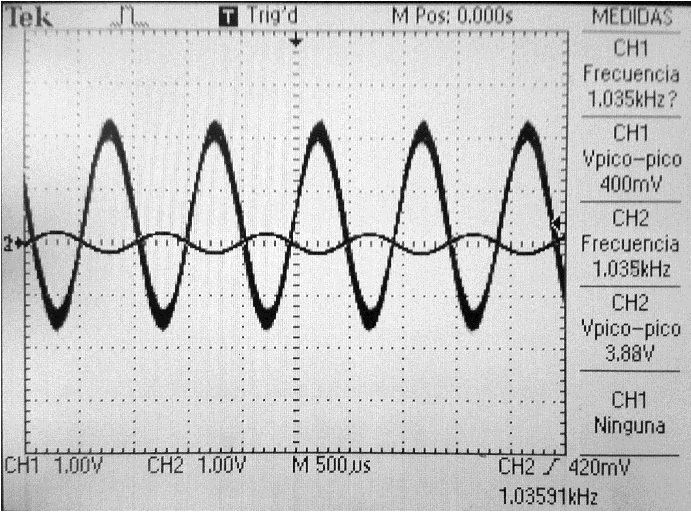
\includegraphics[width=350pt, height=250pt]{mediciones/A1b.jpg}
    \caption{Medición de la tensión de salida}
    \label{fig:vo_med_1b}
    \end{figure}

    Previo a la medición se esperaba encontrar ruido en la misma, debido a las resistencias
    de valor elevado utilizadas, ya que corrientes parásitas generan una caída de tensión
    alta entre los bornes de las resistencias. Para este caso, la amplificación seguirá
    siendo de -10 al igual que en el inciso anterior. De la figura \ref{fig:vo_med_1b} se
    observa lo que se había esperado previamente. Esto se refleja en el ancho de la señal, que representa ruido de frecuencias mayores a $1\,\unit{KHz}$. En este caso el valor pico medido aproximadamente es de $1.99\,\unit{V}$, valor muy cercano al obtenido mediante el modelo ideal. Respecto a la ganancia, la medida fue de -9.95, valor muy próximo al ideal -10. \\

    \item $R_1 = 1\,\unit{K\Omega}$ $R_2 = 1\,\unit{M\Omega}$
    
    Mediantes la ecuaciones \ref{eq:amplificador} y \ref{eq:gan_amplificador} se obtiene $\overset{\wedge}{V}_o = 200\,\unit{V}$ y $A_v$=-1000
    
    Simulando en \emph{Spice} se obtiene la señal de salida mostrada en la figura \ref{fig:vo_1c}. Se observa que si bien la amplificación tiene un valor de -1000, en la
    salida no se ve reflejada ya que los operacionales están alimentados con $\pm 12\, \unit{V}$, lo que limita la tensión de salida.\\
    
    \begin{figure}[H]
    \centering
    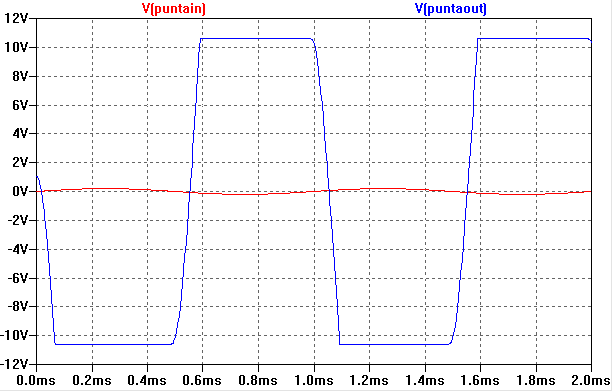
\includegraphics[scale=0.8]{simulaciones/A1C.png}
    \caption{Simulación de la tensión de salida con $A_v = 1000$}
    \label{fig:vo_1c}
    \end{figure}
    
    \begin{figure}[H]
    \centering
    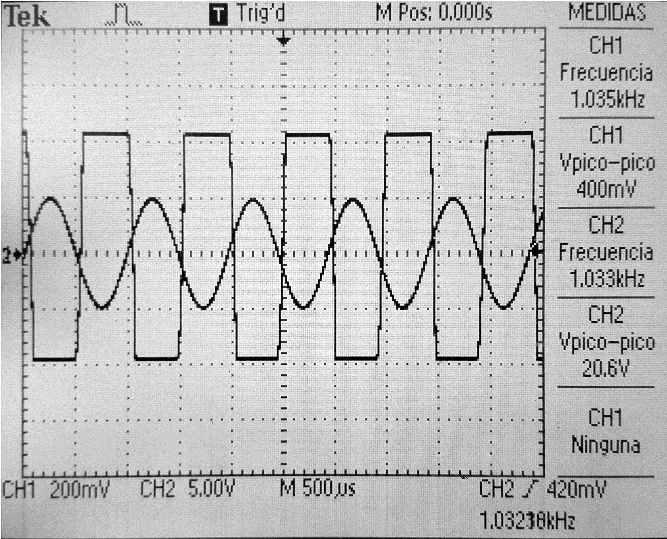
\includegraphics[width=350pt, height=250pt]{mediciones/A1c.jpg}
    \caption{Medición de la tensión de salida con $A_v = 1000$}
    \label{fig:vo_med_1c}
    \end{figure}
    
    
    No se observan diferencias significativas entre la simulación \ref{fig:vo_1c} y la medición \ref{fig:vo_med_1c}, ya que el valor picó de tensión de la simulación fue de $10.6\,\unit{V}$ y el de la medición de $10.3\,\unit{V}$. Respecto a la ganancia la simulada fue de -53 mientras que la medida de -51.5. Acá se observa una gran diferencia respecto al valor ideal que vale -1000. Esto se debe a que la tensión de salida se ve limitada por la alimentación de los AO.
    
    \begin{table}[H]
    \centering
    \begin{tabular}{|c|c|c|c|} %aca pones la cantidad de columnas, te faltaba 1. la c indica que esta centrado el dato en su celda y las | son cada linea vertical de la tabla
    \hline
    Inciso & $\overset{\wedge}{V}_{ideal} [\unit{V}]$ & $\overset{\wedge}{V}_{simulado}[\unit{V}]$ &  $\overset{\wedge}{V}_{medido}[\unit{V}]$ \\ \hline
    a & 2 & 1.90 & 1.99 \\ \hline
    b & 2 & - & 1.99 \\ \hline
    c & 200  & 10.6 & 10.3 \\ \hline
    \end{tabular}
    \caption{Tabla comparativa de valores pico}
    \label{table:tabla_vpico}
    \end{table}
    
    \begin{table}[H]
    \centering
    \begin{tabular}{|c|c|c|c|} %aca pones la cantidad de columnas, te faltaba 1. la c indica que esta centrado el dato en su celda y las | son cada linea vertical de la tabla
    \hline
    Inciso & ${A}_{videal}$ & ${A}_{vsimulado}$ &  ${A}_{vmedido}$  \\ \hline
    a & -10 & -9.5  & -9.04  \\ \hline
    b & -10 & - & -9.95 \\ \hline
    c & -1000 & -53 & -51.5 \\ \hline
    \end{tabular}
    \caption{Tabla comparativa de ganancias}
    \label{table:tabla_ganancia}
    \end{table}

    
    Para obtener los valores picos simulados de la tabla \ref{table:tabla_vpico} se utilizaron las siguientes directivas de LTSpice:
    
    % todo lo que es codigo ponelo entre un verbatim para cambiar la fuente de la letra a una de codigo
    \begin{verbatim}
    .meas Vmax MAX V(PuntaOut) from 0 to 1m
    .meas Vmin MIN V(PuntaOut) from 0 to 1m
    \end{verbatim}

    Con la primera se obtiene el valor máximo durante un periodo, y con la segunda el valor
    mínimo durante el mismo periodo. Luego se realizó la siguiente operación:
    
        
    %si pones ecuaciones que no queres referenciar despues, y las pones en una linea aparte te conviene escribirlas entre un \[ \displaystyle "aca va la ecuacion \] asi queda mas chetito    
        
    \[ \displaystyle \overset{\wedge}{V}_{simulado} = \frac{V_{max}-V_{min}}{2} \]
        
    
    \end{enumerate}

{\color{OliveGreen}
Observar que en el caso b) su valor se aparta más que en a) del predicho por el modelo ideal, al comenzar a influir el valor de la ${R}_{i}$ del AO.}

Esto puede observarse en la medición hecha para el caso b) en la figura \ref{fig:vo_med_1b}. El motivo de lo observado es que el AO LM741 posee una resistencia de entrada de $R_i = 2\,\unit{M\Omega}$, entonces al utilizar una resistencia de valor comparable, como en este caso $R_1 = 1\,\unit{M\Omega}$, el AO deja de comportarse como propone su modelo ideal, es decir, deja de suponer una impedancia de entrada que tiende a infinito.

{\color{OliveGreen}
Para el caso b) modificar la base de tiempo hasta determinar cual es la fuente de ruido que enmascara el valor útil a medir.}

Se modificó la base de tiempo y se determinaron distintas fuentes de ruido. Una de ellas es
la red eléctrica (ver figura \ref{fig:1b_ruido}), la otra se debe a diversos agentes y puede
observarse en la figura \ref{fig:1b_ruido2}. En esta ultima el ruido tiene una frecuencia aproximadamente de  $40\,\unit{KHz}$. \\

\begin{figure}[H]
    \centering
    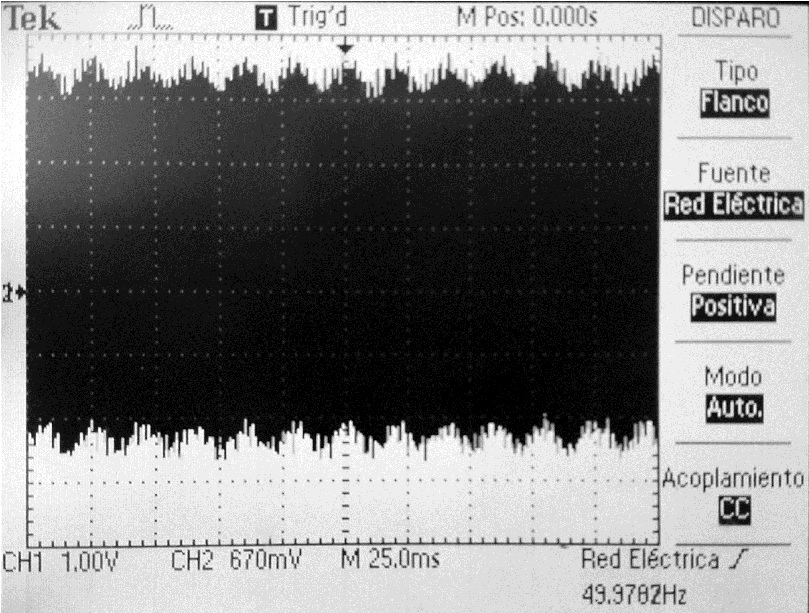
\includegraphics[width=350pt, height=250pt]{mediciones/A1b-ruido.jpg}
    \caption{Medicion del ruido de la tensión de salida introducido por la red eléctrica}
    \label{fig:1b_ruido}
    \end{figure}
    
\begin{figure}[H]
    \centering
    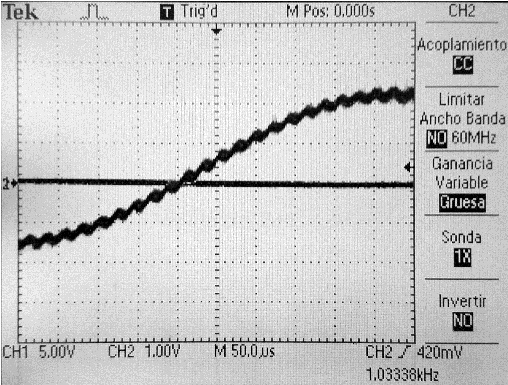
\includegraphics[width=350pt, height=250pt]{mediciones/A1b-ruido2.jpg}
    \caption{Medicion del ruido de la tensión de introducido por otros agentes}
    \label{fig:1b_ruido2}
    \end{figure}    

{\color{OliveGreen}
Observar que en el caso c) es imposible amplificar la señal a los valores que predice el modelo lineal, al alcanzarse los niveles máximos de funcionamiento, determinados por los valores de las tensiones de alimentación.}

Tanto en la simulación (figura \ref{fig:vo_1c}), como en las mediciones de laboratorio pudo observarse esto (figura \ref{fig:vo_med_1c}). Notar que en ambos casos la señal se corta antes de llegar a $12\,\unit{V}$ y $-12\,\unit{V}$, valores correspondientes a la tensión de alimentación del AO.

{\color{OliveGreen}
Para el caso a), reemplazar la carga por otra de $10\,\unit{\Omega}$ y ver que, si ${R}_{L}$ se hace comparable con ${R}_{O}$ del AO, el valor de la amplificación de tensión se aparta del predicho por el modelo lineal.}

Al agregar una ${R}_{L}$ de valor similar a ${R}_{O}$, disminuye la amplificación a lazo
abierto por el divisor resistivo que se genera entre ${R}_{L}$ y ${R}_{O}$ (ver figura \ref{fig:1a_Rl=10}), por lo tanto
disminuye la tensión que cae en ${R}_{L}$, lo que resulta en una disminución de la ganancia. 
Por otro lado, la fuente de corriente de salida del AO tiene, en este caso, un valor máximo
de $25 \,\unit{mA}$ lo que hace que a la salida se pueda tener hasta cierto valor máximo de
tensión. En esta configuración, al tener el AO una corriente máxima de salida de 
$25 \,\unit{mA}$ y una $R_L = 10\,\unit{\Omega}$, la tensión máxima que se podrá tener es de
$V_o = 250\,\unit{mV}$. Ver figuras \ref{fig:vo_1a}, \ref{fig:vo_med_1a} (Simulación y medición con $R_L = 1\,\unit{K\Omega}$), \ref{fig:vo_1aRL} 
y \ref{fig:vo_med_1aRL} (Simulación y medición con $R_L = 10\,\unit{\Omega}$).

\begin{figure}[H]
    \centering
    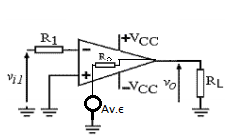
\includegraphics[width=250pt, height=150pt]{circuitos/Circuito_Rl.png}
    \caption{Circuito con ${R}_{L}=10\,\unit{\Omega}$}
    \label{fig:1a_Rl=10}
    \end{figure}




\item  Se obtendrá el valor de $\overset{\wedge}{V}_o$ en vacío para una entrada senoidal con $\overset{\wedge}{V}_{i1}$
entre $50\,\unit{mV}$ y $100\,\unit{mV}$ para $R_1 = 1\,\unit{k\Omega}$ y $R_2 = 10\,\unit{k\Omega}$, variando la frecuencia
del generador de señal de $0\,\unit{Hz}$ a $10\,\unit{MHz}$ 

Para obtener lo pedido se utilizó el siguiente banco de medición:
\begin{figure}[H]
\centering
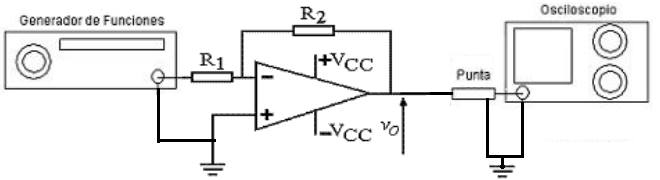
\includegraphics[scale=0.5]{circuitos/A2.png}
\caption{Banco de medición}
\label{fig:banco_de_medicion_A2}
\end{figure}


Se simuló en \emph{Spice} la respuesta en frecuencia de la transferencia del circuito
utilizando punta compensada (figura \ref{fig:2_10x}) y una entrada senoidal de
$75\,\unit{mV}$. Siendo la curva continua la amplitud y la linea punteada la fase. En este
caso siendo la amplificación máxima de $20\,\unit{dB}$ se encontró que la respuesta en frecuencia
alcanza los $17\,\unit{dB}$ en la frecuencia de corte $f_c = 90\,\unit{kHz}$.

En la figura \ref{fig:2_med_10x} puede verse la respuesta en frecuencia representada a partir
de los datos relevados de la medición utilizando punta x10. En este caso la frecuencia de
corte se encuentra entre los $90\,\unit{kHz}$ y los $95\,\unit{kHz}$, lo que coincide con lo
simulado previamente.


\begin{figure}[H]
\centering
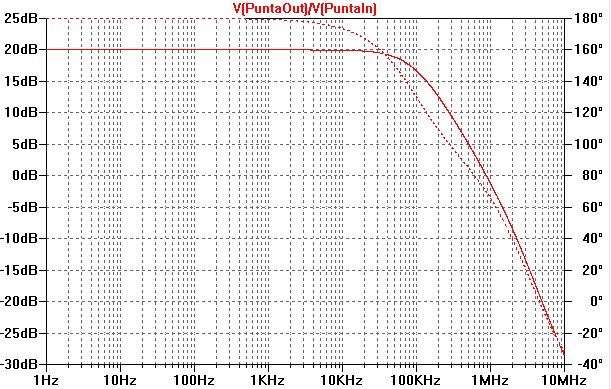
\includegraphics[scale=0.8]{simulaciones/A2puntax10.png}
\caption{Respuesta en frecuencia con punta compensada simulada}
\label{fig:2_10x}
\end{figure}

\begin{figure}[H]
\centering
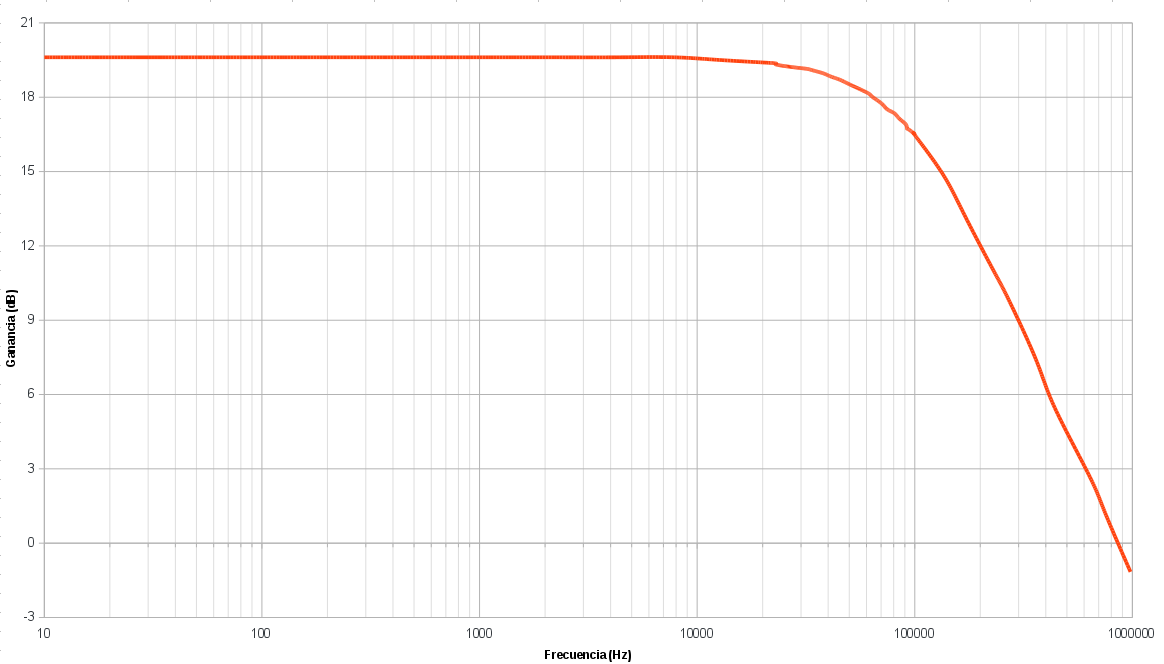
\includegraphics[width=350pt, height=250pt]{mediciones/A2dB_vs_Frec.png}
\caption{Respuesta en frecuencia con punta compensada utilizando datos relevados de la medición}
\label{fig:2_med_10x}
\end{figure}


\begin{figure}[H]
\centering
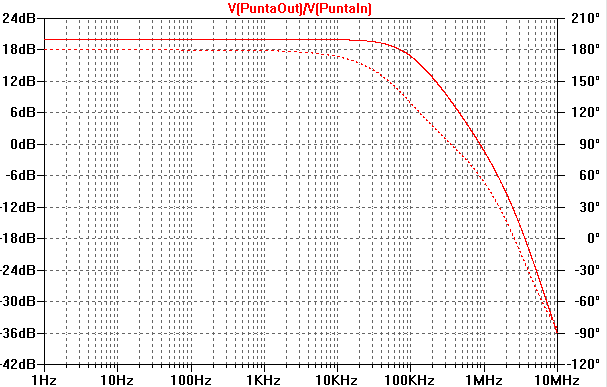
\includegraphics[scale=0.8]{simulaciones/A2puntax1.png}
\caption{Respuesta en frecuencia con punta directa simulada}
\label{fig:2_1x}
\end{figure}

Luego se aumentó la tensión de entrada a $0.5\,\unit{V}$ y se observó que a partir de
frecuencias mayores a $10\,\unit{kHz}$ la señal de salida comienza a deformarse.
En la figura \ref{fig:2_tiempo} se muestran las señales de salida y entrada para una
frecuencia de $50\,\unit{kHz}$ simulada, y en la figura \ref{fig:22_tiempo} las señales de
salida y entrada para la misma frecuencia pero medidas con el osciloscopio.


\begin{figure}[H]
\centering
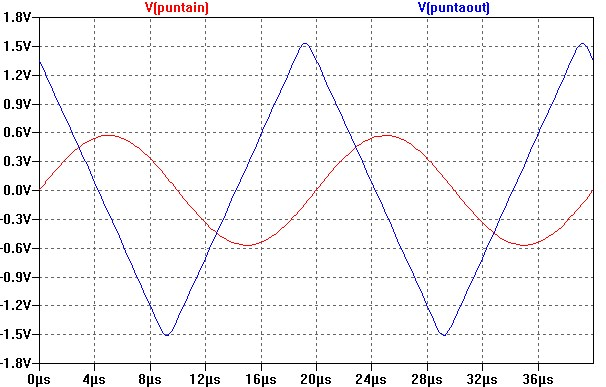
\includegraphics[scale=0.65]{simulaciones/A2sumo0,5V50KHz.png}
\caption{Señal de salida y entrada simulada a $f = 50\,\unit{kHz}$}
\label{fig:2_tiempo}
\end{figure}

\begin{figure}[H]
\centering
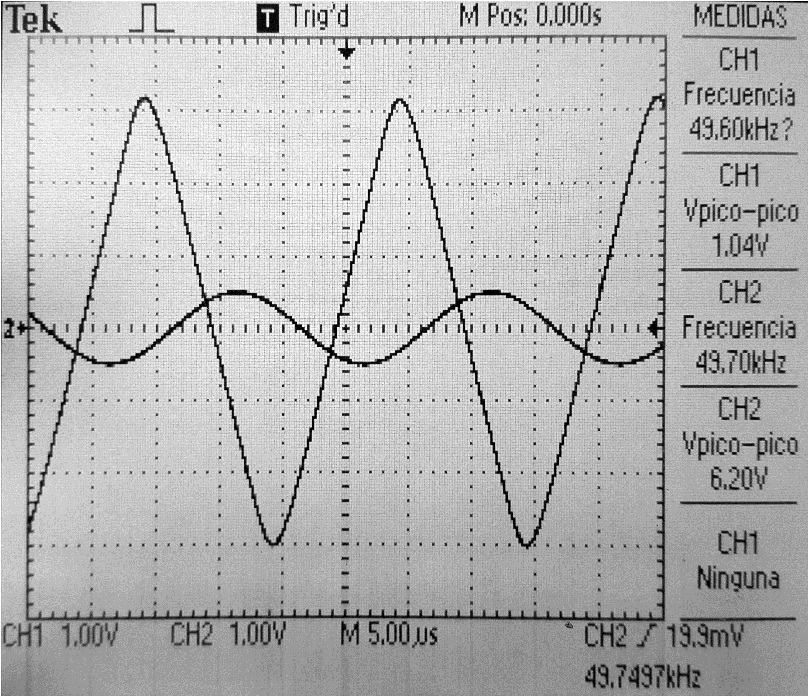
\includegraphics[width=350pt, height=250pt]{mediciones/A2-ultima_preg.jpg}
\caption{Señal de salida y entrada medida a $f = 50\,\unit{kHz}$}
\label{fig:22_tiempo}
\end{figure}


\end{enumerate}

{\color{OliveGreen}¿Se esperaría medir el mismo valor de ${f}_{c}$ de utilizar la punta de
prueba directa (1X)?. ¿Y si se mide con un tester digital?.}\\

Para la punta X1 (ver figura \ref{fig:2_1x}) y X10 se encuentra la misma frecuencia de corte. En el caso
del tester digital (DT830B de la marca UNI-T), al tener un ancho de banda de $45\,\unit{Hz}$
a $400\,\unit{Hz}$ no se lograría medir hasta la frecuencia de corte. Si bien la transferencia del circuito es $T(S) = \frac{-R_2}{R_1}$ no posee ningún polo, las puntas x1 y x10 agreguen capacitores que agregan polos, sin embargo, en las condiciones de trabajo, no modifican la frecuencia de corte.\\

{\color{OliveGreen}Aumentar la tensión a mas de $0.4\,\unit{V}$. Verificar que a partir de de

una frecuencia dada, cambia la forma de la señal de salida. Es decir que para esos niveles de
tensión de entrada y frecuencia, el modelo de amplificador dejaría de predecir correctamente
la forma de la tensión de salida.}\\

Al aumentar la tensión de entrada a más de $0.4\,\unit{V}$, se verifica que para una
frecuencia dada cambia la forma de la señal de salida debido a un efecto no-lineal de los
amplificadores denominado \textquotedblleft slew rate\textquotedblright. Este se define como
el rango máximo de cambio de la
tensión de salida para todas las señales de entrada posibles, por lo que limita la
velocidad de funcionamiento, es decir la frecuencia máxima a la que puede funcionar el
amplificador para un nivel dado de señal de salida. En el AO LM741 la máxima velocidad de
respuesta es $0.5\,\unit{V/\mu s}$. Simulando, se llegó a que para este circuito, la
frecuencia a la que empieza a deformarse la salida es $10\,\unit{KHz}$. Esto puede verse en
la siguiente figura, donde para una entrada senoidal, no se obtiene una salida senoidal perfecta:

\begin{figure}[H]
\centering
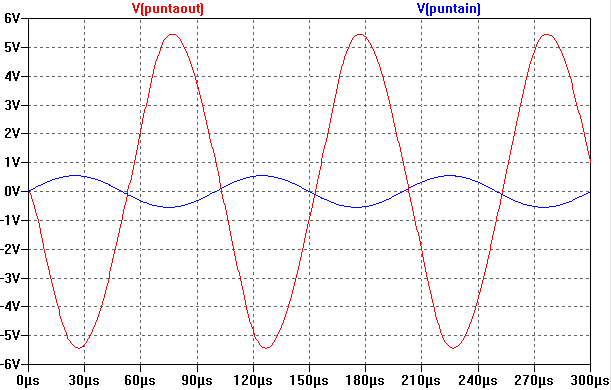
\includegraphics[scale=0.8]{simulaciones/A2sumo0,5V10KHz.png}
\caption{Señal de salida y entrada simulada a $f = 10\,\unit{kHz}$}
\label{fig:A2sumo0,5V10KHz}
\end{figure}

Donde haciendo haciendo \textquotedblleft zoom\textquotedblright a la señal de salida, se
encuentra que el \textquotedblleft slew rate\textquotedblright simulado es aproximadamente de $0.4\,\unit{V/\mu s}$ (es decir, menor a
$0.5\,\unit{V/\mu s}$, valor correspondiente al brindado por la hoja de datos), sin embargo la señal de salida se deforma debido a que los valores que se dan en las hojas de datos de los dispositivos no son exactos, por lo que puede haber cierta dispersión en ellos, y se empezaran a notar los efectos a valores mayores o menores de los brindados por los fabricantes. (ver figura \ref{fig:A2sumo0,5V10KHzZOOM})

\begin{figure}[H]
\centering
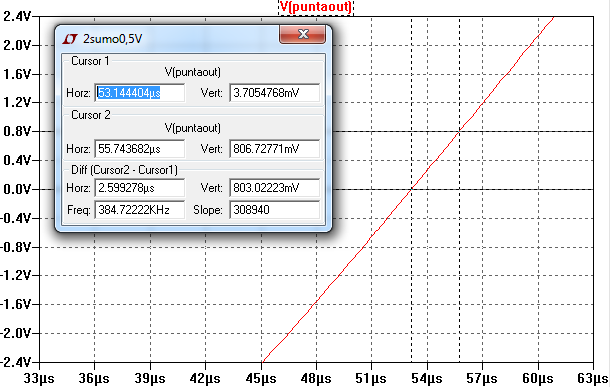
\includegraphics[scale=0.8]{simulaciones/A2sumo0,5V10KHzZOOM.png}
\caption{Zoom de la señal de salida simulada a $f = 10\,\unit{kHz}$}
\label{fig:A2sumo0,5V10KHzZOOM}
\end{figure}




\section{Circuito integrador}

Se utilizará el banco de medición mostrado en la figura \ref{fig:integrador}.
Su tensión de salida se calcula mediante la ecuación \ref{eq:integrador}

\begin{figure}[H]
\centering
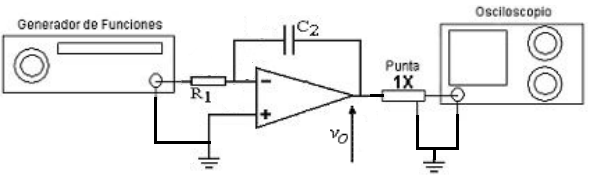
\includegraphics[scale=0.8]{circuitos/BsinR2.png}
\caption{Circuito integrador}
\label{fig:integrador}
\end{figure}



Se utilizará el circuito con la siguiente configuración: Señal de entrada cuadrada de 
$f= \frac{1}{10 \tau}$ y amplitud de $0.2\,\unit{V}$;  $R_1 = 1\,\unit{k\Omega}$ y 
$C_1 = 100\,\unit{nF}$. Para dichos valores la frecuencia resulta $f = 1\,\unit{kHz}$.

Considerando al AO como ideal mediante la ecuación \ref{eq:integrador} se obtiene que 
la señal de salida es una onda triangular de $500\,\unit{mV}$ de amplitud de frecuencia 
$f = 1\,\unit{kHz}$ con componente de continua nula.

Se simuló en \emph{Spice} el circuito integrador utilizando punta directa (figura
\ref{fig:int_x1}) y punta compensada (figura \ref{fig:int_x10}). También se midió el mismo
circuito con punta directa (figura \ref{fig:int_medCC_x1} en CC y figura \ref{fig:int_medCA_x1} en CA) y punta compensada(figura \ref{fig:int_medCC_x10} en CC y figura \ref{fig:int_medCA_x10} en CA).


\begin{figure}[H]
\centering
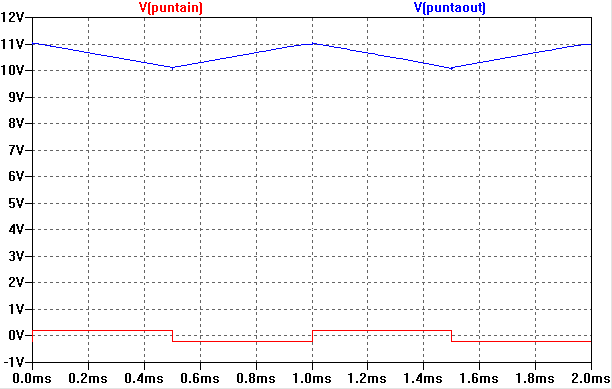
\includegraphics[scale=0.8]{simulaciones/BsinR2puntax1.png}
\caption{Señales de entrada y salida con punta directa simuladas}
\label{fig:int_x1}
\end{figure}

\begin{figure}[H]
\centering
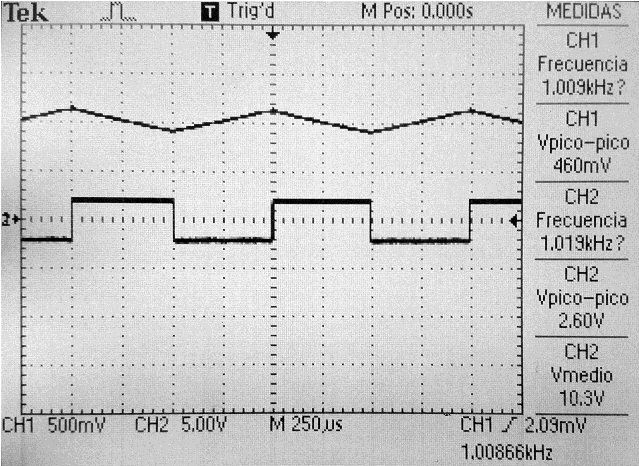
\includegraphics[width=350pt, height=250pt]{mediciones/B-X1-CC.jpg}
\caption{Señales de entrada y salida con punta directa medidas en CC}
\label{fig:int_medCC_x1}
\end{figure}

\begin{figure}[H]
\centering
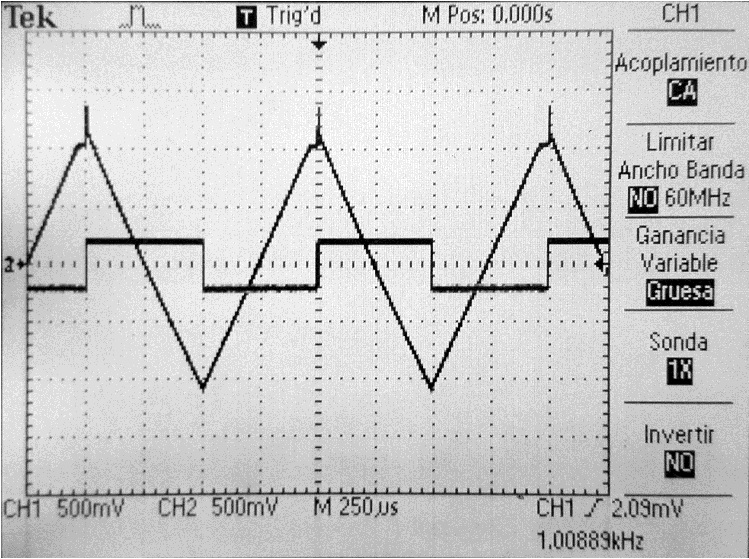
\includegraphics[width=350pt, height=250pt]{mediciones/B-X1-CA.jpg}
\caption{Señales de entrada y salida con punta directa medidas en CA}
\label{fig:int_medCA_x1}
\end{figure}

De las figuras anteriores (figuras \ref{fig:int_x1}, \ref{fig:int_medCC_x1} y \ref{fig:int_medCA_x1}), se obtuvo que el tiempo de crecimiento para la señal de salida de la medición fue $0.40 \unit{ms}$, mientras que el simulado fue $0.42 \unit{ms}$. Estos valores están muy cerca (igual en el caso de la medición) del valor ideal ($0.40 \unit{ms}$). Respecto al valor medio, al medir en CC con el osciloscopio se obtuvo un valor de $10.3 \unit{V}$, mientras que simulando se obtuvo un valor de $10.6 \unit{V}$. Estos valores se alejan mucho del modelo ideal, ya que en este el valor medio es 0. Para corroborar esto, se midió en CA para eliminar la componente de continua y se obtuvo un valor medio muy cercano a 0 (del orden de los $\unit{mV}$). Respecto a la forma de onda, observando las figuras correspondientes a la medición en CC y la simulación no se observan diferencias significativas.

\begin{figure}[H]
\centering
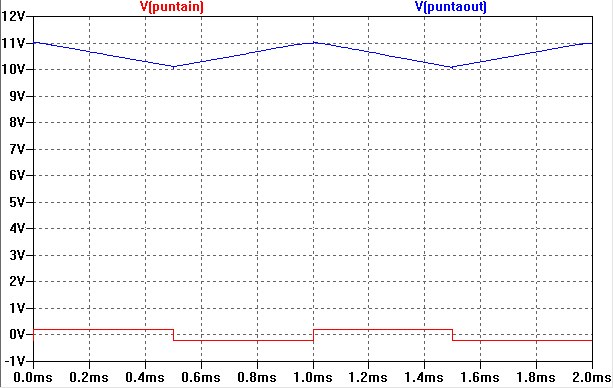
\includegraphics[scale=0.8]{simulaciones/BsinR2puntax10.png}
\caption{Señales de entrada y salida con punta compensada simuladas}
\label{fig:int_x10}
\end{figure}

\begin{figure}[H]
\centering
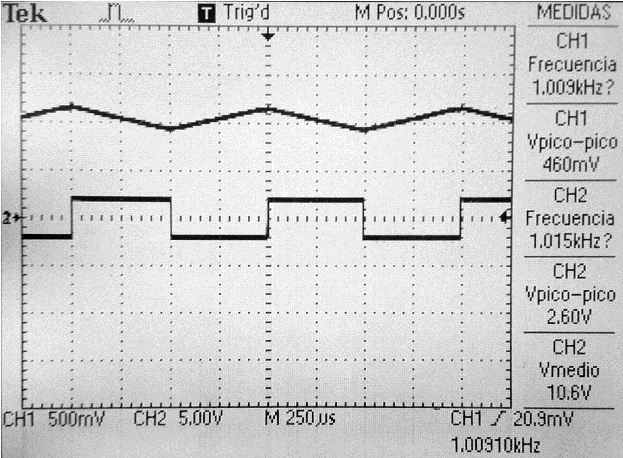
\includegraphics[width=350pt, height=250pt]{mediciones/B-X10-CC.jpg}
\caption{Señales de entrada y salida con punta compensada medidas en CC}
\label{fig:int_medCC_x10}
\end{figure}

\begin{figure}[H]
\centering
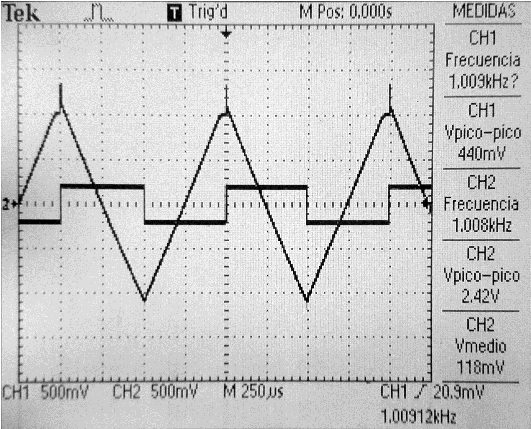
\includegraphics[width=350pt, height=250pt]{mediciones/B-X10-CA.jpg}
\caption{Señales de entrada y salida con punta compensada medidas en CA}
\label{fig:int_medCA_x10}
\end{figure}

De las figuras anteriores (figuras \ref{fig:int_x10}, \ref{fig:int_medCC_x10} y \ref{fig:int_medCA_x10}), se obtuvo que el tiempo de crecimiento para la señal de salida de la medición fue $0.40 \unit{ms}$, mientras que el simulado fue $0.41 \unit{ms}$. Estos valores son muy próximos al valor ideal ($0.40 \unit{ms}$). Respecto al valor medio, al medir en CC con el osciloscopio se obtuvo un valor de $10.6 \unit{V}$, mientras que simulando se obtuvo un valor de $10.6 \unit{V}$. Estos valores se alejan mucho del modelo ideal, ya que en este el valor medio es 0. Midiendo en CA para eliminar la componente de continua, se obtuvo un valor medio de $118 \unit{mV}$. Respecto a la forma de onda, observando la medición en CC y la simulación no se tienen diferencias perceptibles.

No se observaron diferencias significativas entre las mediciones y simulaciones hechas con punta directa, con las hechas con punta compensada en ninguno de los aspectos anteriormente analizados (valor medio, tiempo de crecimiento y forma de onda). \\ 

Se agregó un resistor $R_2 = 10\,\unit{k\Omega}$ en paralelo con $C_2$ y se volvió
a simular con punta directa(figura \ref{fig:int_x1_R}) y con punta compensada(figura \ref{fig:int_x10_R}). Tambien se volvió a medir con punta directa (figura \ref{fig:int_x1_R_med}) y punta compensada (figura \ref{fig:int_x10_R_med}). En estas figuras se puede observar que salida ya no tiene la misma forma de onda que las mediciones en CA hechas anteriormente, ya que la curva se ve mas parecida a una exponencial. Sin embargo disminuye el valor medio, por lo que este caso es el mas parecido al predicho por el modelo ideal (que tiene un valor medio nulo). Nuevamente no se aprecian diferencias perceptibles entre la punta directa y la punta compensada, sin embargo, para ambas puntas, se observa que en la simulación, en los valores pico (tanto positivo como negativo) hay un salto en la tensión (frecuencia alta). Esto no se puede observar en las mediciones ya que ni aunque se use la punta compensada que agranda el ancho de banda del osciloscopio se tiene la posibilidad de medir una frecuencia de tal magnitud.


\begin{figure}[H]
\centering
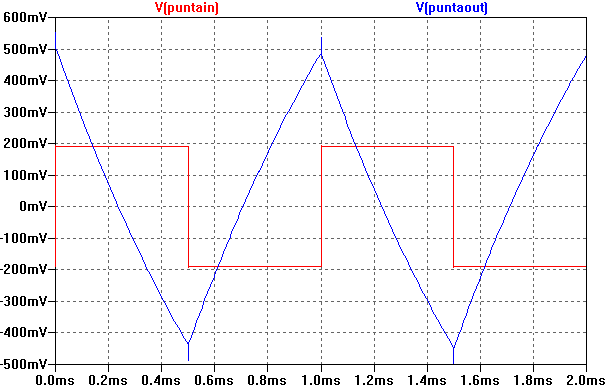
\includegraphics[scale=0.8]{simulaciones/BconR2Puntax1.png}
\caption{Señales de entrada y salida con $R_2$ en paralelo a $C_2$ utilizando punta directa simuladas}
\label{fig:int_x1_R}
\end{figure}

\begin{figure}[H]
\centering
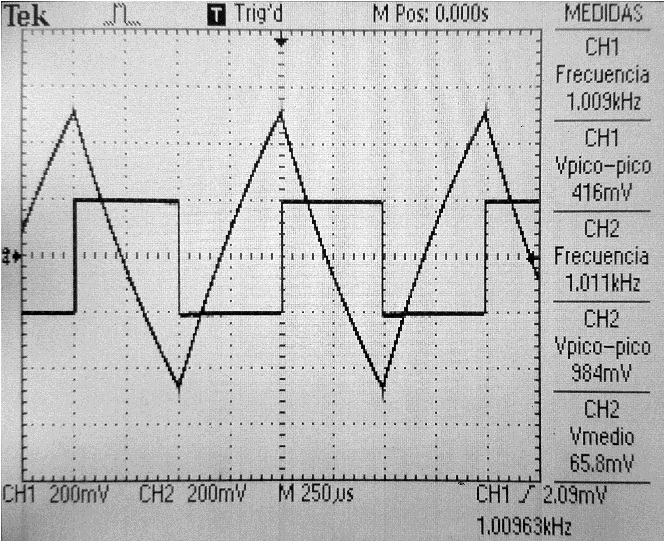
\includegraphics[width=350pt, height=250pt]{mediciones/B-X1-CC-10K.jpg}
\caption{Señales de entrada y salida con $R_2$ en paralelo a $C_2$ utilizando punta directa medidas}
\label{fig:int_x1_R_med}
\end{figure}

\begin{figure}[H]
\centering
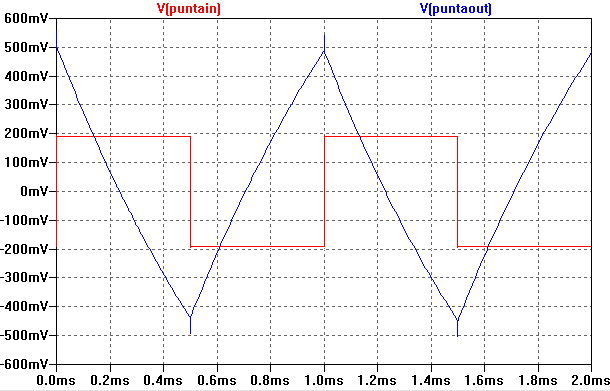
\includegraphics[scale=0.8]{simulaciones/BconR2puntax10.png}
\caption{Señales de entrada y salida con $R_2$ en paralelo a $C_2$ utilizando punta compensada simuladas}
\label{fig:int_x10_R}
\end{figure}

\begin{figure}[H]
\centering
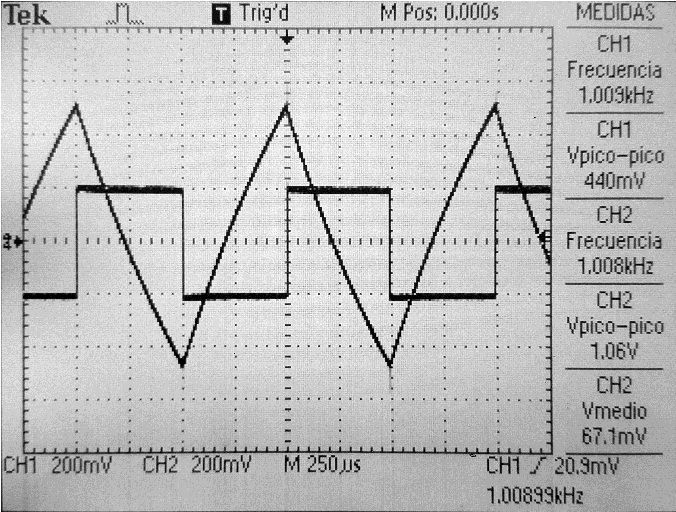
\includegraphics[width=350pt, height=250pt]{mediciones/B-X10-CC-10K.jpg}
\caption{Señales de entrada y salida con $R_2$ en paralelo a $C_2$ utilizando punta compensada medidas}
\label{fig:int_x10_R_med}
\end{figure}



\begin{table}[H]
\centering
\begin{tabular}{|c|c|} \hline
Inciso & ${t}_{r}[\unit{ms}]$   \\ \hline
Teórico & 0.40  \\ \hline
Simulacion x1 & 0.42  \\ \hline
Medición x1 & 0.40 \\ \hline
Simulación x10 & 0.41 \\ \hline
Medición x10 & 0.40 \\ \hline
\end{tabular}
\caption{Tabla comparativa de tiempos de crecimiento sin la resistencia ${R}_{2}$}
\label{table:tabla_tcrecimiento}
\end{table}

\begin{table}[H]
\centering
\begin{tabular}{|c|c|} \hline
Inciso & ${V}_{medio}[\unit{V}]$   \\ \hline
Teórico & 0 \\ \hline
Simulacion x1 & 10.6 \\ \hline
Medición x1 & 10.3 \\ \hline
Simulación x10 & 10.6 \\ \hline
Medición x10 & 10.6 \\ \hline
\end{tabular}
\caption{Tabla comparativa de valores medios sin la resistencia ${R}_{2}$}
\label{table:tabla_vmedio}
\end{table}

En la tabla \ref{table:tabla_tcrecimiento} se observan los tiempos de crecimiento de cada tensión de salida. El tiempo de crecimiento se define como el tiempo que tarda una señal en pasar del 10\% de la misma al 90\%. Para el caso de la simulación este se obtuvo utilizando las siguientes directivas de \emph{Spice}:
\begin{verbatim}
.meas Vpp PP V(PuntaOut) from 0ms to 1ms
.meas Vmin MIN V(PuntaOut) from 0 to 1m
\end{verbatim}
Siendo V(PuntaOut) la tensión en la salida. Con la primer directiva se obtuvo el valor pico a
pico, y con la segunda el valor mínimo, ambas durante un periodo. Luego se hicieron las siguientes cuentas:\\
$V_{10\%}$ = $V_{min}$ + 0.1*$_{Vpp}$\\
$V_{90\%}$ = $V_{min}$+ 0.9*$V_{pp}$\\
Una vez que se obtuvieron estos valores, se utilizaron los cursores de LTSpice posicionando
el cursor 2 en la tensión $V_{90\%}$ y el cursor 1 en la tensión $V_{10\%}$. Esta ventana
indica cuanto vale la resta de los tiempos correspondientes al cursor 2 y cursor 1, dando
esto como resultado el tiempo de crecimiento.\\
En la misma tabla se pueden observar los valores correspondientes a las mediciones, estos fueron calculados observando la pantalla del osciloscopio.\\
Para calcular el valor teórico del tiempo de crecimiento, como se dijo anteriormente, considerando al AO como ideal y utilizando la ecuación \ref{eq:integrador} se obtiene que 
la señal de salida es una onda triangular de $500\,\unit{mV}$ de amplitud y de frecuencia 
$f = 1\,\unit{kHz}$ con componente de continua nula. Teniendo esta señal, se calculó la recta con pendiente positiva (tiempo en donde la cuadrada de entrada es negativa):\\
$V_{out}$(t)=2000*t -1.5\\
Con esta recta, se calcularon los tiempos donde la señal alcanza el 10\% y el 90\% de la misma, es decir $-400\,\unit{mV}$ y $400\,\unit{mV}$. Utilizando estas tensiones en la ecuación anterior, se obtiene que $t_{10\%}$=$0.55\,\unit{ms}$ y $t_{90\%}$=$0.95\,\unit{ms}$. Haciendo la resta se obtiene que $t_{r}$=$0.4\,\unit{ms}$.\\

En la tabla \ref{table:tabla_vmedio} se observan los valores medios de la señal de salida. Para la simulación se utilizó la directiva:
\begin{verbatim}
.meas Vmedio AVG V(PuntaOut) from 0ms to 1ms
\end{verbatim}
Esta indica el valor medio durante un periodo de la señal V(PuntaOut), que en este caso corresponde a la señal de salida. Los valores medios de las mediciones fueron obtenidos configurando los cursores del osciloscopio. El valor medio teórico vale 0 ya que se esta integrando una señal cuadrada, y se compensan las áreas.\\


{\color{OliveGreen}Observar que la integración se ve limitada por los niveles máximos de funcionamiento dados por las tensiones de alimentación.}

Esto se debe a que, si se plantea la transferencia del circuito (mediante Laplace), se observa que en $s=0$ se tiene un polo, lo que implica que cuando la tensión de entrada sea constante (frecuencia nula), se obtiene una ganancia infinita, es decir, la salida tiende a infinito. En la practica, la salida esta limitada por la saturación del AO, que está dada por su alimentación, en este caso,  $\pm 12\, \unit{V}$. Si a la entrada no se tuviera ninguna continua, igualmente saturaría a $+V_{cc}$ o $-V{cc}$ debido a la tensión de offset que tiene el operacional en sus terminales. Esta tensión al ir integrándose va sumando una componente de continua que terminaría haciendo saturar la señal a $+V_{cc}$  o $-V{cc}$.\\

{\color{OliveGreen}Agregar un resistor $R_2 = 10\,\unit{K\Omega}$ en paralelo con $C_2$ y observar que la descarga de $C_2$ a través de $R_2$ permite un funcionamiento cercano al predicho en el modelo ideal, evitando alcanzar los límites de niveles de tensión de funcionamiento.}
 
Al agregar $R_2$ se permite la descarga de $C_2$ a través de dicha resistencia y se evita alcanzar los limites de niveles de tensión de funcionamiento, ya que se limita la ganancia. 
Es decir que en este caso, planteando la transferencia, se observa que el polo que antes estaba en $s=0$ se desplaza hacia $s= \frac{-1}{R_2 C_2}$, por lo que para la continua (frecuencia nula) no se tiene ganancia infinita y se evita llegar a la tensión de saturación del AO, siendo esta su tensión de alimentación, que en este caso es $\pm 12\, \unit{V}$.

%-----------------------------------------------------------------------------
%------------------------ RECTIFICADOR SIMPLE --------------------------------
%-----------------------------------------------------------------------------

\section{Circuitos Rectificadores}

\subsection{Rectificador Simple}

El circuito rectificador de media onda que se muestra en el banco de medición de la figura \ref{fig:rect_banco}, implementado con un diodo 1N4001/07 y un resistor $R_L = 10\,\unit{k\Omega}$, es excitado por una señal senoidal de frecuencia $f = 50\,\unit{Hz}$ y amplitud $\overset{\wedge}{V}_{i} = 5\,\unit{V}$.\\

{\color{OliveGreen}¿Por qué se utiliza una amplitud pico de $5\,\unit{V}$ en la excitación y no de $50\,\unit{mV}$?}\\

Se utiliza una alimentación de $5\,\unit{V}$ ya que si se utilizara una excitación de $50\,\unit{mV}$ el diodo no estaría en directa ya que debe superar la tensión umbral\footnote{Dato obtenido en la hoja de datos del componente, ver referencia \cite{Diodo 1N4001/07}} ($V_T = 0.7\,\unit{V}$), y no se obtendría ninguna tensión a la salida. 

\begin{figure}[H]
\centering
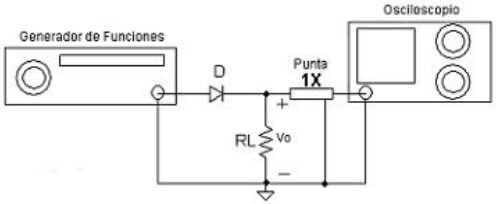
\includegraphics[scale=0.8]{circuitos/Fsincap.png}
\caption{Banco de medición}
\label{fig:rect_banco}
\end{figure}

Mediante el modelo teórico del diodo se calcula la tensión pico de la salida, esta se alcanza cuando la señal de entrada alcanza su valor máximo:

\[\displaystyle \overset{\wedge}{V}_{o} = \overset{\wedge}{V}_{i} - V_T = 5\,\unit{V} - 0.7\,\unit{V} = 4.3\,\unit{V} \]

Luego se aproxima el valor medio\footnote{Se despreció para este calculo el intervalo en el que la señal de entrada aún no supera $V_T$, debiendo ser nula la salida en este intervalo, quedando media onda senoidal de $f=50\,\unit{Hz}$} de una media onda senoidal partiendo de su definición:

\[ \displaystyle \overset{-}{V}_{o} = \frac{1}{T}\int_0^T V_o(t) dt = \frac{1}{T} \left( \int_0^{T/2} \overset{\wedge}{V}_{o} sen(w t) dt  + \int_{T/2}^{T} 0 dt \right) = \frac{1}{T} \int_0^{T/2} \overset{\wedge}{V}_{o} sen(w t) dt \]

\[ \displaystyle  = \frac{\overset{\wedge}{V}_{o}}{T} \left[\frac{-cos(wt)}{w}  \right]^{T/2}_0 = \frac{\overset{\wedge}{V}_{o}}{T w} \left[-cos\left(\frac{wT}{2}\right) + cos(0) \right]\]

Reemplazando $T = \frac{1}{f}$ y $w = 2 \pi f$ en el desarrollo se obtiene:

\[ \displaystyle \overset{-}{V}_{o} = \frac{\overset{\wedge}{V}_{o} f}{2 \pi f} \left[-cos\left(\frac{2 \pi f}{f 2}\right) + cos(0) \right] = \frac{\overset{\wedge}{V}_{o}}{2 \pi} \left[-cos(\pi) + cos(0) \right] = \frac{\overset{\wedge}{V}_{o}}{2 \pi} \left[1 + 1 \right] = \frac{\overset{\wedge}{V}_{o} 2}{2 \pi} = \frac{\overset{\wedge}{V}_{o}}{\pi}\]

Por lo tanto:

\begin{equation}
    \overset{-}{V}_{o} = \frac{\overset{\wedge}{V}_{o}}{\pi}
    \label{eq:Vmedio}
\end{equation}

Mediante la ecuación \ref{eq:Vmedio} se obtiene que:

\[ \displaystyle \overset{-}{V}_{o} \approx \frac{4.3\,\unit{V}}{\pi} \approx 1.369 \]


Simulando en \emph{Spice} se obtuvo la señal de salida mostrada en la figura \ref{fig:F_50_sim}. Resultando $\overset{-}{V}_{o} = 1.34381 \,\unit{V} $ y
$\overset{\wedge}{V}_{o} = 4.44365 \,\unit{V} $

\begin{figure}[H]
\centering
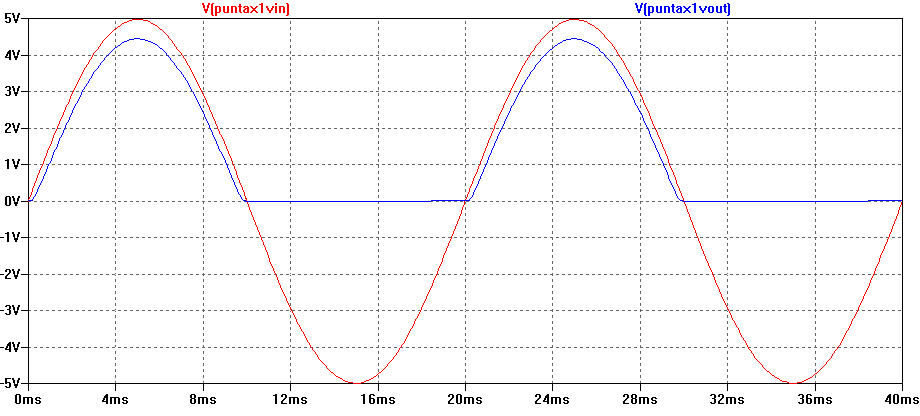
\includegraphics[scale=0.65]{simulaciones/F_vo_50.png}
\caption{Simulación con $f = 50\,\unit{Hz}$}
\label{fig:F_50_sim}
\end{figure}

En la figura \ref{fig:F_50_med} se muestran la señal de entrada y salida de la mediciones realizadas. Obteniéndose $\overset{-}{V}_{o} = 1.42 \,\unit{V} $ y $\overset{\wedge}{V}_{o} = 4.56 \,\unit{V} $

\begin{figure}[H]
\centering
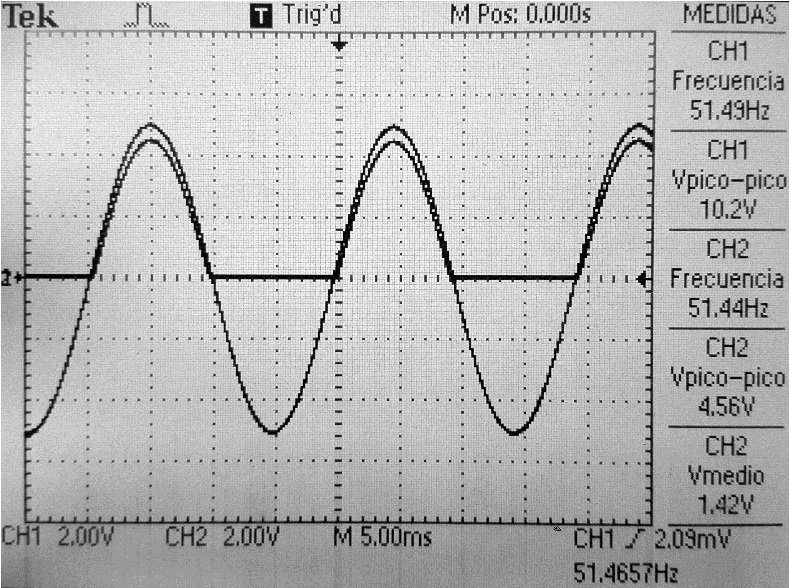
\includegraphics[width=350pt, height=250pt]{mediciones/F-50Hz.jpg}
\caption{Medición con $f = 50\,\unit{Hz}$}
\label{fig:F_50_med}
\end{figure}

A continuación, en la tabla \ref{table:F_50} se resume en una tabla los valores obtenidos para cada método:

\begin{table}[H]
\centering
\begin{tabular}{|c|c|c|}
\hline
Método     & $\overset{-}{V}_{o} [\unit{V}] $  & $\overset{\wedge}{V}_{o} [\unit{V}]$ \\ \hline
Cálculo    & 1.37                   & 4.30  \\ \hline
Simulación & 1.34                   & 4.44  \\ \hline
Medición   & 1.42                   & 4.56  \\ \hline
\end{tabular}
\caption{Tabla comparativa de los resultados obtenidos}
\label{table:F_50}
\end{table}

En la tabla \ref{table:F_50_errores} se muestran los errores obtenidos
al obtener los valores mediante cálculo y simulación respecto a la medición.
En donde no se obtuvieron errores altos para ambos métodos.

\begin{table}[H]
\centering
\begin{tabular}{|c|c|c|}
\hline
Método     & Error de $\overset{-}{V}_{o}$  & Error de $\overset{\wedge}{V}_{o}$ \\ \hline
Cálculo    & $-3.52 \unit{\%} $             & $-5.70 \unit{\%} $  \\ \hline
Simulación & $-5.63 \unit{\%} $             & $-2.63 \unit{\%} $  \\ \hline
\end{tabular}
\caption{Tabla de errores respecto a los valores medidos}
\label{table:F_50_errores}
\end{table}

Seguidamente, se conecta un capacitor $C = 47\,\unit{\mu F}$ en paralelo con $R_L$. Se lo
excitará con una señal senoidal de frecuencia $50\,\unit{Hz}$ y amplitud $5\,\unit{V}$ pico.
Como se muestra en el banco de medición de la figura \ref{fig:rect_banco_C}

\begin{figure}[H]
\centering
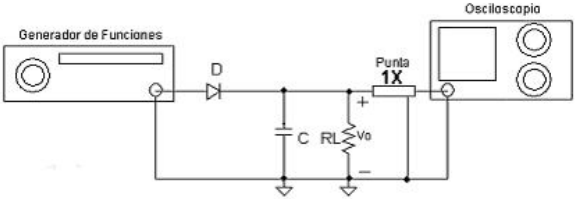
\includegraphics[scale=0.6]{circuitos/Fconcap.png}
\caption{Banco de medición}
\label{fig:rect_banco_C}
\end{figure}


A continuación se muestran los resultados obtenidos simulando en \emph{Spice}
y en las mediciones del laboratorio, para distintos valores de $R_L$.


\begin{itemize}
    \item $\overset{-}{V_o}$: Valor medio 
    \item $V_{ripple}$: La variación máxima de tensión de salida (ripple).
    Se obtendrá mediante $V_{ripple} = \Delta V_o$. 
    \item $z_{\%}$: Es el \textbf{porcentaje de ripple} o \textbf{rizado}.
    Se calculará mediante la siguiente ecuación:

    \begin{equation}
        z_{\%} = 100 \frac{V_{ripple}}{\overset{-}{V_o}}
        \label{eq:z_ripple}
    \end{equation}

\end{itemize}



\begin{enumerate}
    \item $R_L = 10\,\unit{k\Omega}$
    
    En las figuras \ref{fig:F1_10k_cc_sim} y \ref{fig:F1_10k_cc_med} se muestran las señales de entrada
    y salida obtenidas en modo CC mediante simulación y medición respectivamente. 

    \begin{figure}[H]
    \centering
    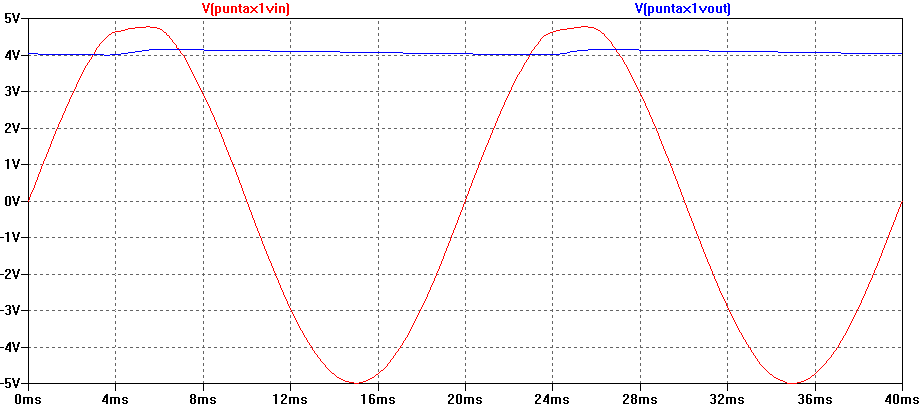
\includegraphics[scale=0.65]{simulaciones/F1_vo_RL-10k.png}
    \caption{Señal de salida simulada con $R_L = 10\,\unit{k\Omega}$}
    \label{fig:F1_10k_cc_sim}
    \end{figure}
    
    \begin{figure}[H]
    \centering
    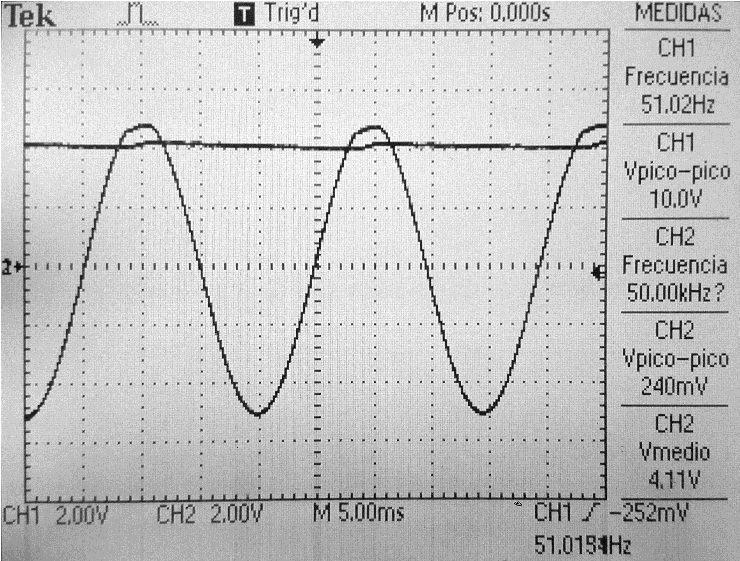
\includegraphics[width=350pt, height=250pt]{mediciones/F1-10K.jpg}
    \caption{Señal de salida medida con $R_L = 10\,\unit{k\Omega}$ en modo CC}
    \label{fig:F1_10k_cc_med}
    \end{figure}
    
    En la figura \ref{fig:F1_10k_ca_sim} se muestra un zoom de la señal de salida simulada y en
    la figura \ref{fig:F1_10k_ca_med} se muestra la señal de salida medida en modo CA.
    
    \begin{figure}[H]
    \centering
    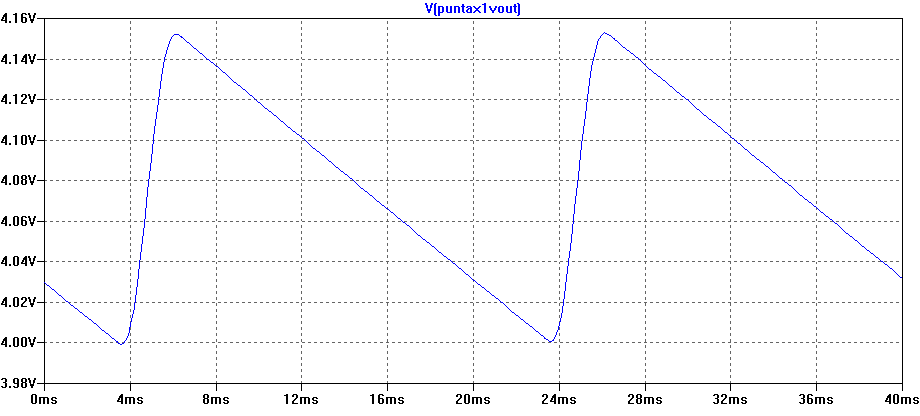
\includegraphics[scale=0.65]{simulaciones/F1_vo_RL-10k_zoom.png}
    \caption{Zoom de la señal de salida simulada con $R_L = 10\,\unit{k\Omega}$}
    \label{fig:F1_10k_ca_sim}
    \end{figure}
    
    \begin{figure}[H]
    \centering
    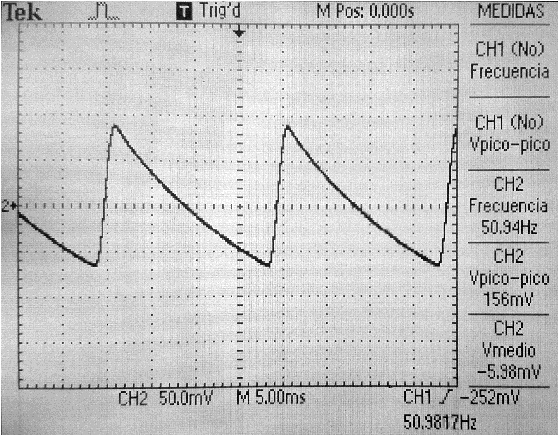
\includegraphics[width=350pt, height=250pt]{mediciones/F1-10K-CA.jpg}
    \caption{Señal de salida medida con $R_L = 10\,\unit{k\Omega}$ en modo CA}
    \label{fig:F1_10k_ca_med}
    \end{figure}
    
%   --------------- 4k7 ---------------------------------------------    
    

    \item $R_L = 4.7\,\unit{k\Omega}$
    
    En las figuras \ref{fig:F1_4k7_cc_sim} y \ref{fig:F1_4k7_cc_med} se muestran las señales de entrada
    y salida obtenidas en modo CC mediante simulación y medición respectivamente. 

    \begin{figure}[H]
    \centering
    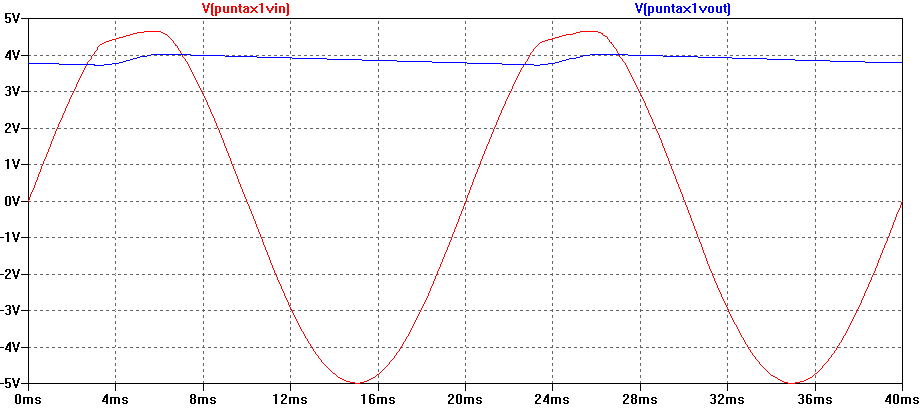
\includegraphics[scale=0.65]{simulaciones/F1_vo_RL-4k7.png}
    \caption{Señal de salida simulada con $R_L = 4.7\,\unit{k\Omega}$}
    \label{fig:F1_4k7_cc_sim}
    \end{figure}
    
    \begin{figure}[H]
    \centering
    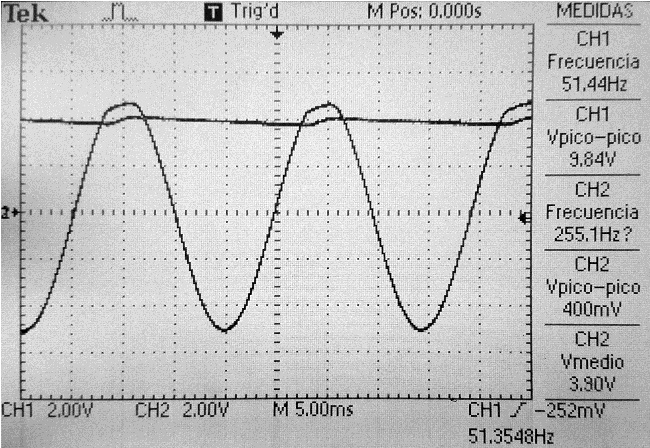
\includegraphics[width=350pt, height=250pt]{mediciones/F1-4K7.jpg}
    \caption{Señal de salida medida con $R_L = 4.7\,\unit{k\Omega}$ en modo CC}
    \label{fig:F1_4k7_cc_med}
    \end{figure}
    
    En la figura \ref{fig:F1_4k7_ca_sim} se muestra un zoom de la señal de salida simulada y en
    la figura \ref{fig:F1_4k7_ca_med} se muestra la señal de salida medida en modo CA.
    
    \begin{figure}[H]
    \centering
    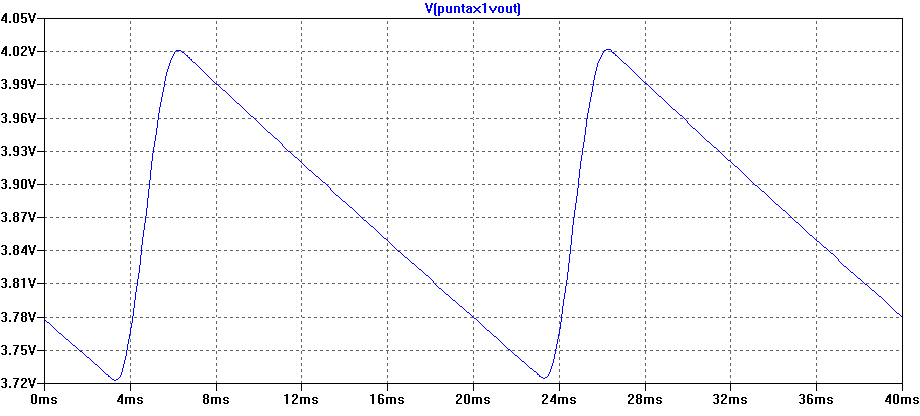
\includegraphics[scale=0.65]{simulaciones/F1_vo_RL-4k7_zoom.png}
    \caption{Zoom de la señal de salida simulada con $R_L = 4.7\,\unit{k\Omega}$}
    \label{fig:F1_4k7_ca_sim}
    \end{figure}
    
    \begin{figure}[H]
    \centering
    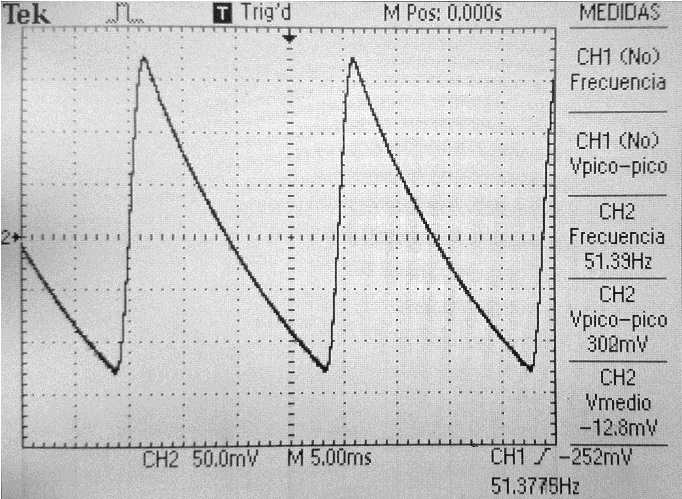
\includegraphics[width=350pt, height=250pt]{mediciones/F1-4K7-CA.jpg}
    \caption{Señal de salida medida con $R_L = 4.7\,\unit{k\Omega}$ en modo CA}
    \label{fig:F1_4k7_ca_med}
    \end{figure}
    
    % --------------------------- 1k ---------------------------------------
    
    \item $R_L = 1\,\unit{k\Omega}$
    
    En las figuras \ref{fig:F1_1k_cc_sim} y \ref{fig:F1_1k_cc_med} se muestran las señales de entrada
    y salida obtenidas en modo CC mediante simulación y medición respectivamente. 

    \begin{figure}[H]
    \centering
    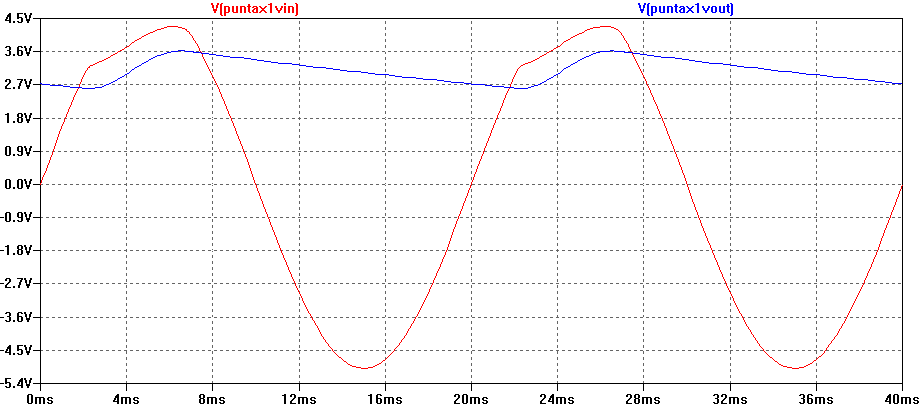
\includegraphics[scale=0.65]{simulaciones/F1_vo_RL-1k.png}
    \caption{Señal de salida simulada con $R_L = 1\,\unit{k\Omega}$ en modo CC}
    \label{fig:F1_1k_cc_sim}
    \end{figure}
    
    \begin{figure}[H]
    \centering
    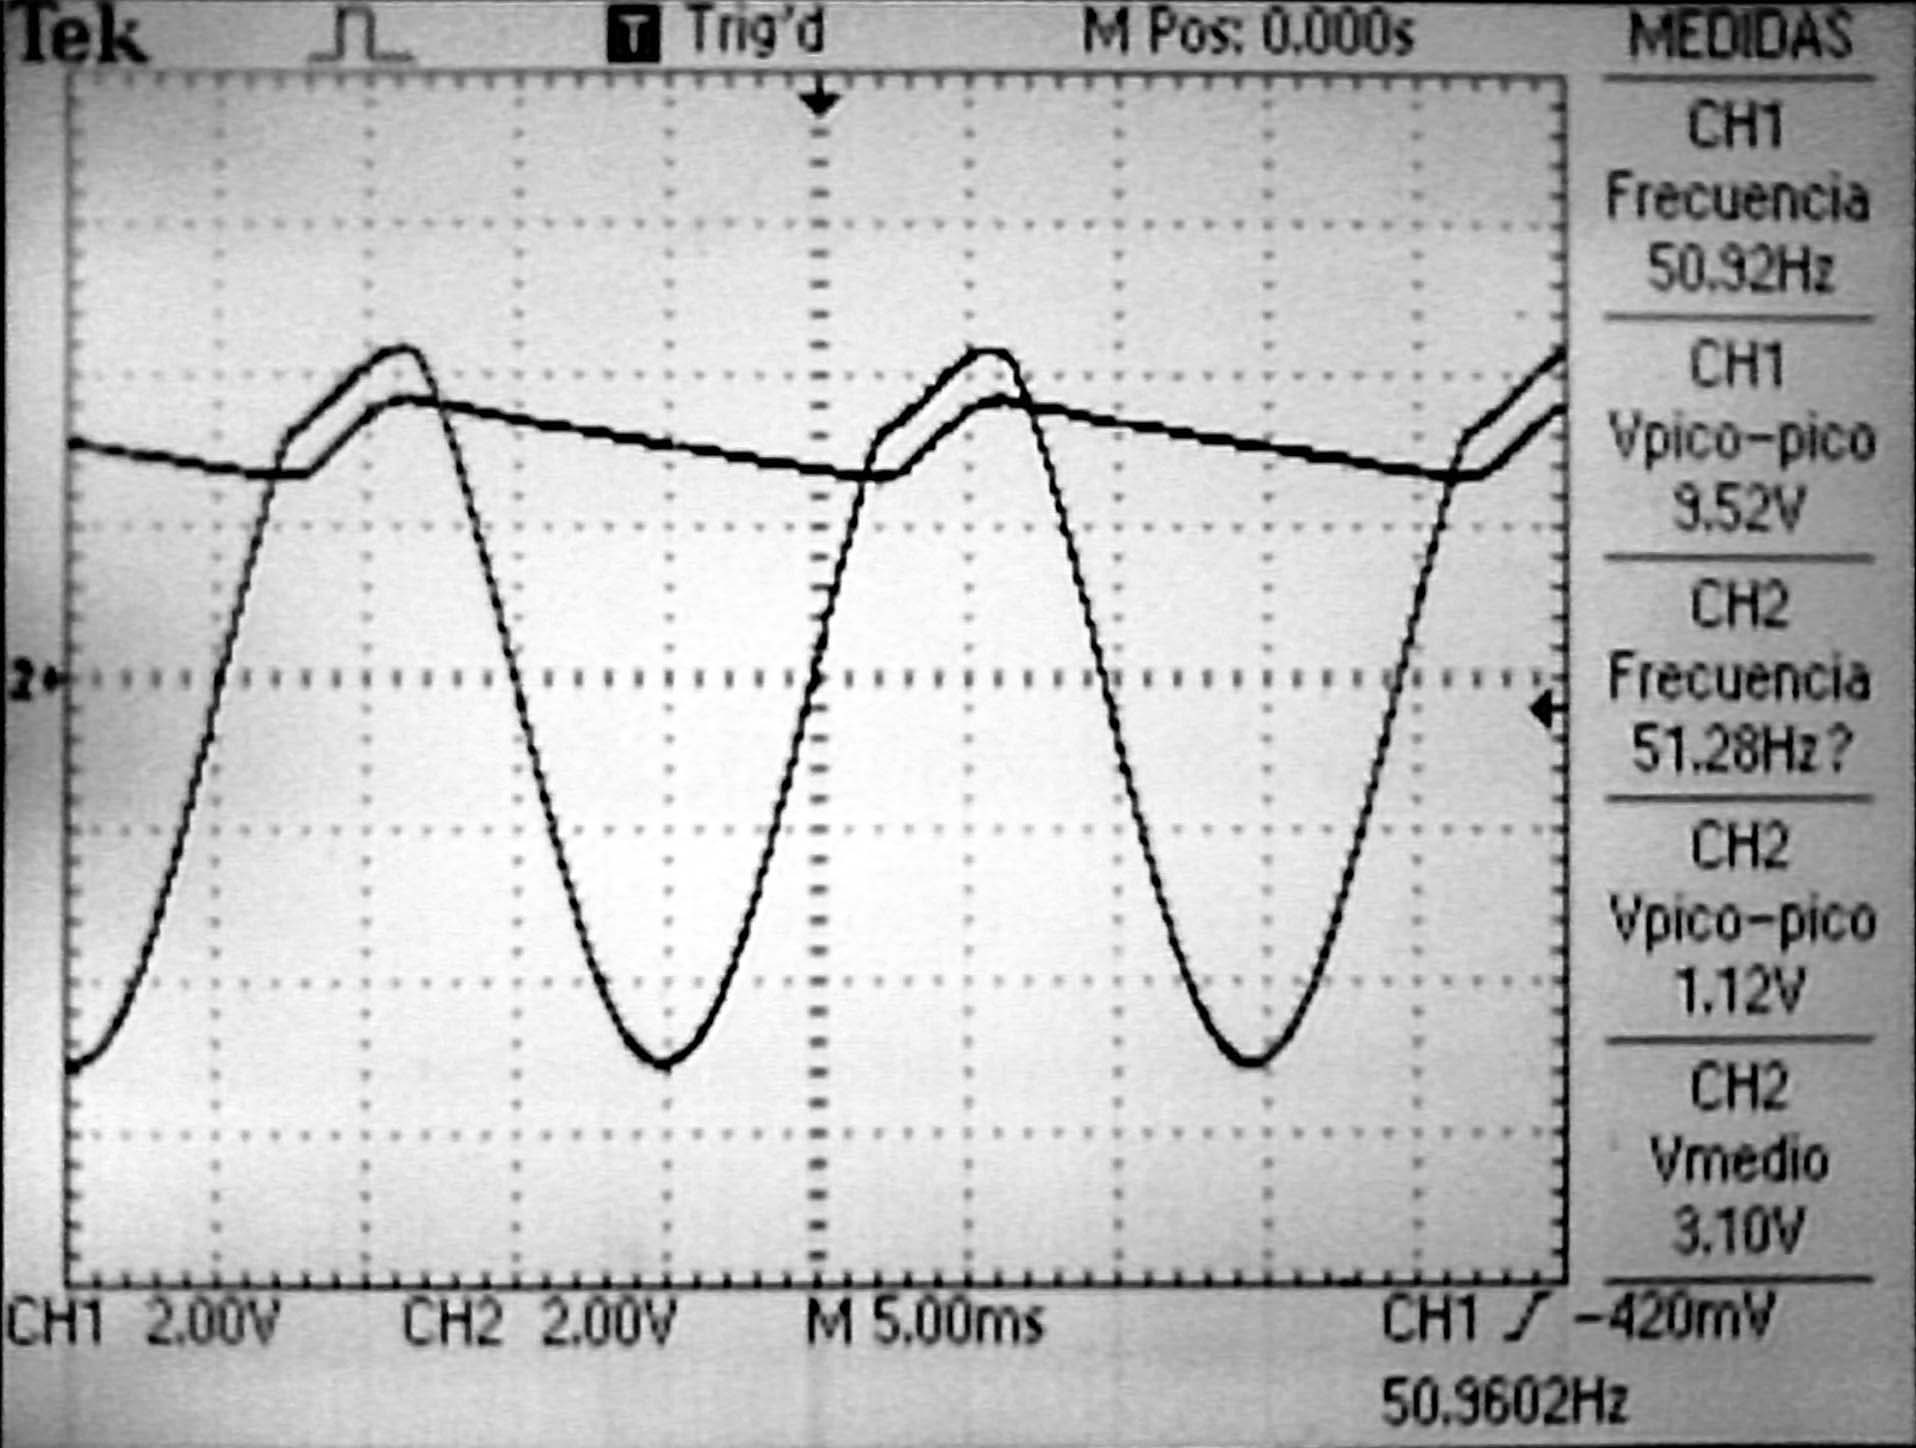
\includegraphics[width=350pt, height=250pt]{mediciones/F1-1K.jpg}
    \caption{Señal de salida medida con $R_L = 1\,\unit{k\Omega}$}
    \label{fig:F1_1k_cc_med}
    \end{figure}
    
    En la figura \ref{fig:F1_1k_ca_sim} se muestra un zoom de la señal de salida simulada y en
    la figura \ref{fig:F1_1k_ca_med} se muestra la señal de salida medida en modo CA.
    
    \begin{figure}[H]
    \centering
    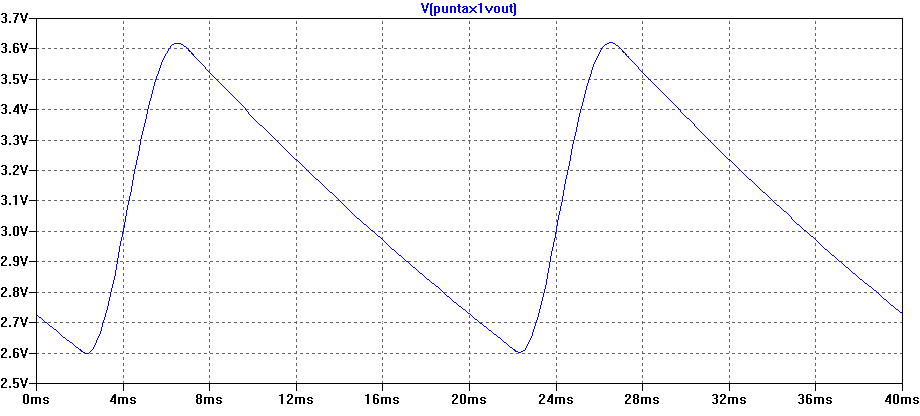
\includegraphics[scale=0.65]{simulaciones/F1_vo_RL-1k_zoom.png}
    \caption{Señal de salida simulada con $R_L = 1\,\unit{k\Omega}$ en modo CA}
    \label{fig:F1_1k_ca_sim}
    \end{figure}
    
    \begin{figure}[H]
    \centering
    \includegraphics[width=350pt, height=250pt]{mediciones/F1-1K-CA.jpg}
    \caption{Zoom de la señal de salida medida con $R_L = 1\,\unit{k\Omega}$}
    \label{fig:F1_1k_ca_med}
    \end{figure}
    
\end{enumerate}

En todas las mediciones se encontró que la señal de entrada estaba deformada en sus picos positivos.
Esto se debe a que cuando el diodo se activa, comienza a circular corriente que carga al capacitor.
Esta corriente origina una caída de tensión en la resistencia interna del generador de señales, que
es de $50\,\unit{\Omega}$. El capacitor tiene una reactancia de $67.73\,\unit{\Omega}$ por lo que 
es comparable con la resistencia interna del generador.
Mientras menor es $R_L$ esta deformación es mas notoria, ya que
al disminuir $R_L$ el capacitor se descarga mas rápido al estar desactivado el diodo y por lo tanto
al activarse el diodo circula más corriente para cargar al capacitor.

En la tabla \ref{table:F1_z_ripple} se resumen los datos obtenidos para cada método y cada $R_L$. Calculando $z_{\%}$ mediante la ecuación \ref{eq:z_ripple}

\begin{table}[H]
\centering
\begin{tabular}{c|c|c|c|c|}
\cline{2-5}
& Método     &  $\overset{-}{V}_{o}$  & ${V}_{ripple}$ & $z_{\%}$ \\ \hline

\multicolumn{1}{|c|}{\multirow{2}{*}{$R_L = 10\,\unit{k\Omega}$}} & Simulación & $4.08\,\unit{V}$ & $153\,\unit{mV}$ & $3.75\,\unit{\%}$ \\ \cline{2-5}
\multicolumn{1}{|c|}{} & Medición & $4.11\,\unit{V}$ & $156\,\unit{mV}$ & $3.80\,\unit{\%}$     \\ \hline

\multicolumn{1}{|c|}{\multirow{2}{*}{$R_L = 4.7\,\unit{k\Omega}$}} & Simulación & $3.87\,\unit{V}$ & $298\,\unit{mV}$ & $7.70\,\unit{\%}$ \\ \cline{2-5}
\multicolumn{1}{|c|}{} & Medición & $3.90\,\unit{V}$ & $302\,\unit{mV}$ & $7.74\,\unit{\%}$   \\ \hline

\multicolumn{1}{|c|}{\multirow{2}{*}{$R_L = 1\,\unit{k\Omega}$}} & Simulación & $3.10\,\unit{V}$ & $1.02\,\unit{V}$ & $32.9\,\unit{\%}$ \\ \cline{2-5}
\multicolumn{1}{|c|}{} & Medición & $3.10\,\unit{V}$ & $1.04\,\unit{V}$ & $33.5\,\unit{\%}$     \\ \hline

\end{tabular}
\label{table:F1_z_ripple}
\end{table}


Con los datos obtenidos se representó la característica de regulación en la figura \ref{fig:F1_caracteristica_regulacion} utilizando los datos de las mediciones y simulaciones.

\begin{figure}[H]
\centering
\includegraphics[width=350pt, height=250pt]{mediciones/F1.png}
\caption{Característica de regulación}
\label{fig:F1_caracteristica_regulacion}
\end{figure}


{\color{OliveGreen} ¿Para que sirve la curva denominada \textquotedblleft
característica de regulación\textquotedblright?}

Sirve para obtener la relación entre el valor medio de la tensión de salida
$\overset{-}{V}_{o}$ en relación con la resistencia de carga $R_L$. Para
así conocer que resistencia de carga debe ser conectada para obtener
un determinado $\overset{-}{V}_{o}$.

{\color{Orange} Si en lugar de un rectificador de media onda se tuviese un puente rectificador de onda completa, ¿se esperaría un $z_{\%}$ mayor o menor?}

Se esperaría un $z_{\%}$ menor, ya que $\overset{-}{V}_{o}$ aumentaría
y $V_{ripple}$ disminuiría. Ya que al ser de onda completa, el área bajo su curva aumentaría y por lo tanto aumenta $\overset{-}{V}_{o}$ y al reducirse el tiempo entre los picos de la curva de salida, disminuye $V_{ripple}$.

%-----------------------------------------------------------------------------
%------------------ RECTIFICADOR DE PRECISIÓN --------------------------------
%-----------------------------------------------------------------------------

\subsection{Rectificador de media onda de precisión}

Se utilizó el banco de medición mostrado en la figura \ref{fig:4_circuito} es excitado por una señal senoidal de frecuencia $f = 50\,\unit{Hz}$ y amplitud $\overset{\wedge}{V}_{i} = 5\,\unit{V}$


\begin{figure}[H]
\centering
\includegraphics[scale=0.7]{circuitos/Fprecision.png}
\caption{Circuito rectificador de media onda de precisión}
\label{fig:4_circuito}
\end{figure}


Simulando en \emph{Spice} se obtuvo la señal de salida mostrada en la figura 
\ref{fig:F4_50_sim}. Obteniéndose un valor pico de $ \overset{\wedge}{V}_{o} = -4.96\,\unit{V} $ 
y un valor medio de $\overset{-}{V}_{o} = -1.58\,\unit{V}$

\begin{figure}[H]
\centering
\includegraphics[scale=0.65]{simulaciones/F4_vo_50.png}
\caption{Simulación con $f=50\,\unit{Hz}$}
\label{fig:F4_50_sim}
\end{figure}

Luego en las mediciones del laboratorio se obtuvo la señal de salida mostrada
en la figura \ref{fig:F4_50_med}. Obteniéndose un valor pico de 
$\overset{\wedge}{V}_{o} = -5.04\,\unit{V}$ y un valor medio de $\overset{-}{V}_{o} = -1.36\,\unit{V}$

\begin{figure}[H]
\centering
\includegraphics[width=350pt, height=250pt]{mediciones/F4-50Hz.jpg}
\caption{Medición con $f=50\,\unit{Hz}$}
\label{fig:F4_50_med}
\end{figure}


A continuación, en la tabla \ref{table:F_40} se resume en una tabla los
valores obtenidos mediante simulación y medición:

\begin{table}[H]
\centering
\begin{tabular}{|c|c|c|}
\hline
Método     & $\overset{-}{V}_{o} [\unit{V}] $  & $\overset{\wedge}{V}_{o} [\unit{V}]$ \\ \hline
Simulación & -1.58                 & -4.96  \\ \hline
Medición   & -1.36                    & -5.04                   \\ \hline
\end{tabular}
\caption{Tabla comparativa de los resultados obtenidos}
\label{table:F_40}
\end{table}

A continuación se listan los errores de las simulaciones respecto a las mediciones:

\begin{itemize}
    \item Error de $\overset{-}{V}_{o}$:  $ 16.2\,\unit{\%} $
    \item Error de $\overset{\wedge}{V}_{o}$:  $1.59\,\unit{\%} $
\end{itemize}

Seguidamente, se conecta un capacitor $C = 47\,\unit{\mu F}$ en paralelo con 
$R_L$. Utilizando el banco de medición mostrado en la figura \ref{fig:F4_banco_C}

\begin{figure}[H]
\centering
\includegraphics[scale=0.65]{circuitos/FprecisionC.png}
\caption{Banco de medición}
\label{fig:F4_banco_C}
\end{figure}


A continuación se muestran los resultados obtenidos simulando en \emph{Spice}
y en las mediciones del laboratorio, para distintos valores de $R_L$.


\begin{itemize}
    \item $\overset{-}{V_o}$: Valor medio 
    \item $V_{ripple}$: La variación máxima de tensión de salida (ripple).
    Se obtendrá mediante $V_{ripple} = \Delta V_o$. 
    \item $z_{\%}$: Es el \textbf{porcentaje de ripple} o \textbf{rizado}.
    Se calculará mediante la siguiente ecuación:

    \begin{equation}
        z_{\%} = 100 \frac{V_{ripple}}{\overset{-}{V_o}}
        \label{eq:z_ripple}
    \end{equation}

\end{itemize}



\begin{enumerate}
    \item $R_L = 10\,\unit{k\Omega}$
    
    En las figuras \ref{fig:F4_10k_cc_sim} y \ref{fig:F4_10k_cc_med} se muestran las señales de entrada
    y salida obtenidas en modo CC mediante simulación y medición respectivamente. 

    \begin{figure}[H]
    \centering
    \includegraphics[scale=0.65]{simulaciones/F4_vo_RL-10k.png}
    \caption{Señal de salida simulada con $R_L = 10\,\unit{k\Omega}$}
    \label{fig:F4_10k_cc_sim}
    \end{figure}
    
    \begin{figure}[H]
    \centering
    \includegraphics[width=350pt, height=250pt]{mediciones/F4-10K.jpg}
    \caption{Señal de salida medida con $R_L = 10\,\unit{k\Omega}$ en modo CC}
    \label{fig:F4_10k_cc_med}
    \end{figure}
    
    En la figura \ref{fig:F4_10k_ca_sim} se muestra un zoom de la señal de salida simulada y en
    la figura \ref{fig:F4_10k_ca_med} se muestra la señal de salida medida en modo CA.

    
    \begin{figure}[H]
    \centering
    \includegraphics[scale=0.65]{simulaciones/F4_vo_RL-10k_zoom.png}
    \caption{Zoom de la señal de salida simulada con $R_L = 10\,\unit{k\Omega}$}
    \label{fig:F4_10k_ca_sim}
    \end{figure}
    
    \begin{figure}[H]
    \centering
    \includegraphics[width=350pt, height=250pt]{mediciones/F4-10K-CA.jpg}
    \caption{Señal de salida medida con $R_L = 10\,\unit{k\Omega}$ en modo CA}
    \label{fig:F4_10k_ca_med}
    \end{figure}
    
%   --------------- 4k7 ---------------------------------------------    
    

    \item $R_L = 4.7\,\unit{k\Omega}$
    
    En las figuras \ref{fig:F4_4k7_cc_sim} y \ref{fig:F4_4k7_cc_med} se muestran las señales de entrada
    y salida obtenidas en modo CC mediante simulación y medición respectivamente. 

    \begin{figure}[H]
    \centering
    \includegraphics[scale=0.65]{simulaciones/F4_vo_RL-4k7.png}
    \caption{Señal de salida simulada con $R_L = 4.7\,\unit{k\Omega}$}
    \label{fig:F4_4k7_cc_sim}
    \end{figure}
    
    \begin{figure}[H]
    \centering
    \includegraphics[width=350pt, height=250pt]{mediciones/F4-4K7.jpg}
    \caption{Señal de salida medida con $R_L = 4.7\,\unit{k\Omega}$ en modo CC}
    \label{fig:F4_4k7_cc_med}
    \end{figure}
    
    
    En la figura \ref{fig:F4_4k7_ca_sim} se muestra un zoom de la señal de salida simulada y en
    la figura \ref{fig:F4_4k7_ca_med} se muestra la señal de salida medida en modo CA.
    
    \begin{figure}[H]
    \centering
    \includegraphics[scale=0.65]{simulaciones/F4_vo_RL-4k7_zoom.png}
    \caption{Zoom de la señal de señal de salida simulada con $R_L = 4.7\,\unit{k\Omega}$}
    \label{fig:F4_4k7_ca_sim}
    \end{figure}
    
    \begin{figure}[H]
    \centering
    \includegraphics[width=350pt, height=250pt]{mediciones/F4-4K7-CA.jpg}
    \caption{Señal de salida medida con $R_L = 4.7\,\unit{k\Omega}$ en modo CA}
    \label{fig:F4_4k7_ca_med}
    \end{figure}
    
    % --------------------------- 1k ---------------------------------------
    
    \item $R_L = 1\,\unit{k\Omega}$
    
    En las figuras \ref{fig:F4_1k_cc_sim} y \ref{fig:F1_4k_cc_med} se muestran las señales de entrada
    y salida obtenidas en modo CC mediante simulación y medicion respectivamente. 

    \begin{figure}[H]
    \centering
    \includegraphics[scale=0.65]{simulaciones/F4_vo_RL-1k.png}
    \caption{Señal de salida simulada con $R_L = 1\,\unit{k\Omega}$}
    \label{fig:F4_1k_cc_sim}
    \end{figure}
    
    \begin{figure}[H]
    \centering
    \includegraphics[width=350pt, height=250pt]{mediciones/F4-1K.jpg}
    \caption{Señal de salida medida con $R_L = 1\,\unit{k\Omega}$ en modo CC}
    \label{fig:F1_4k_cc_med}
    \end{figure}
    
    En la figura \ref{fig:F4_1k_ca_sim} se muestra un zoom de la señal de salida simulada y en
    la figura \ref{fig:F4_1k_ca_med} se muestra la señal de salida medida en modo CA.
    
    \begin{figure}[H]
    \centering
    \includegraphics[scale=0.65]{simulaciones/F4_vo_RL-1k_zoom.png}
    \caption{Zoom de la señal de señal de salida simulada con $R_L = 1\,\unit{k\Omega}$}
    \label{fig:F4_1k_ca_sim}
    \end{figure}
    
    \begin{figure}[H]
    \centering
    \includegraphics[width=350pt, height=250pt]{mediciones/F4-1K-CA.jpg}
    \caption{Señal de salida medida con $R_L = 1\,\unit{k\Omega}$ en modo CA}
    \label{fig:F4_1k_ca_med}
    \end{figure}
    
\end{enumerate}


En la tabla \ref{table:F4_z_ripple} se resumen los datos obtenidos para cada método y cada $R_L$. Calculando $z_{\%}$ mediante la ecuación \ref{eq:z_ripple}

\begin{table}[H]
\centering
\begin{tabular}{c|c|c|c|c|}
\cline{2-5}
& Método     &  $\overset{-}{V}_{o}$  & ${V}_{ripple}$ & $z_{\%}$ \\ \hline

\multicolumn{1}{|c|}{\multirow{2}{*}{$R_L = 10\,\unit{k\Omega}$}} & 
Simulación & $-4.80\,\unit{V}$ & $387\,\unit{mV}$ & $8.06\,\unit{\%}$ \\ \cline{2-5}
\multicolumn{1}{|c|}{} & 
Medición & $-4.70\,\unit{V}$ & $392\,\unit{mV}$ & $8.34\,\unit{\%}$     \\ \hline

\multicolumn{1}{|c|}{\multirow{2}{*}{$R_L = 4.7\,\unit{k\Omega}$}} & 
Simulación & $-4.69\,\unit{V}$ & $588\,\unit{mV}$ & $12.5\,\unit{\%}$ \\ \cline{2-5}
\multicolumn{1}{|c|}{} & 
Medición & $-4.58\,\unit{V}$ & $564\,\unit{mV}$ & $12.31\,\unit{\%}$   \\ \hline

\multicolumn{1}{|c|}{\multirow{2}{*}{$R_L = 1\,\unit{k\Omega}$}} & 
Simulación & $-4.00\,\unit{V}$ & $1.53\,\unit{V}$ & $38.3\,\unit{\%}$ \\ \cline{2-5}
\multicolumn{1}{|c|}{} & 
Medición & $-3.95\,\unit{V}$ & $1.66\,\unit{V}$ & $42.03\,\unit{\%}$     \\ \hline
\end{tabular}
\label{table:F4_z_ripple}
\end{table}


Con los datos obtenidos se representó la característica de regulación en la figura \ref{fig:F4_caracteristica_regulacion} utilizando los datos de las mediciones y simulaciones.

\begin{figure}[H]
\centering
\includegraphics[width=350pt, height=250pt]{mediciones/F4.jpg}
\caption{Característica de regulación}
\label{fig:F4_caracteristica_regulacion}
\end{figure}



{\color{OliveGreen} ¿Qué sucede si se reemplaza $R_2 = 10\,\unit{k\Omega}$
por un resistor de $22\,\unit{k\Omega}$?}


Al reemplazar la resistencia $R_2$ por una de $22\,\unit{k\Omega}$, la tensión de salida en el semiciclo negativo continua valiendo 0, pero en el ciclo positivo
se obtiene una amplificación de $A_v = -\frac{R_2}{R_1} = -\frac{22\,\unit{k\Omega}}{10\,\unit{k\Omega}} = -2.2$ por lo que $V_o=-V_i 2.2$. El circuito corta la señal aproximadamente en $-10\,\unit{V}$ debido a la limitación de tensión en la salida del AO dada por su alimentación de $\pm 12\, \unit{V}$.


En las figuras \ref{fig:F4_22k_sim} y \ref{fig:F4_22k} puede verse la tensión de salida ,simulada y medida, recortada debido a este efecto.


\begin{figure}[H]
\centering
\includegraphics[scale = 0.65]{simulaciones/F4_22k_sim.jpg}
\caption{Señal de salida simulada utilizando $R_2 = 22\,\unit{k\Omega}$}
\label{fig:F4_22k_sim}
\end{figure}


\begin{figure}[H]
\centering
\includegraphics[width=350pt, height=250pt]{mediciones/F4-22k.jpg}
\caption{Señal de salida medida utilizando $R_2 = 22\,\unit{k\Omega}$}
\label{fig:F4_22k}
\end{figure}


{\color{Orange} ¿Qué sucede si se invierte la conexión de cada diodo?}

Al invertir los diodos se obtiene un rectificador de media onda positiva. Sin capacitor en paralelo a
$R_L$ la señal de salida vale 0 cuando la señal de entrada es positiva y vale un semiciclo positivo de un seno cuando la señal de entrada es negativa. Esto ocurre debido a que cuando la señal de entrada es positiva el diodo $D_2$ se activa y el diodo $D_1$ se desactiva, por lo que la señal de salida es nula ya
que no circula corriente por $R_2$. Y cuando la señal de entrada es negativa el diodo $D_2$ se desactiva y el diodo $D_1$ se activa, por lo que circulará corriente por $R_2$ y por lo tanto habrá tensión en la salida.

\subsection{Comparación de Rectificadores}

La principal diferencia entre los rectificadores analizados, es que el rectificador de precisión puede
rectificar pequeñas señales debido a que no se requiere tensión de entrada para activar los diodos.

La salida del rectificador simple es la señal de entrada rectificada menos la tensión umbral del diodo: $V_{i rect} - V_T$. Mientras que en el rectificador de precisión la señal de salida es igual a la señal de entrada rectificada. Debido a esto y a que la tensión de entrada debe superar la tensión umbral del diodo, el rectificador simple tendrá menor área bajo su curva de salida y por lo tanto tendrá un valor medio menor que el del rectificador de precisión.

Se obtuvieron porcentaje de ripple $z_{\%}$ similares para ambos rectificadores, ya que este depende de \\ $\tau = R_L C$ del circuito. Que es el mismo para ambos rectificadores. Ya que $\overset{-}{V}_{o}$ es mayor para los rectificadores de precisión y $z_{\%}$ es igual para ambos rectificadores; $V_{ripple}$
del rectificador de precisión debe ser mayor al del rectificador simple.

Para ambos rectificadores se obtuvieron las curvas llamadas \textquotedblleft característica de regulación\textquotedblright con forma de rectas. Logrando la curva del rectificador de precisión tensiones medias mas altas que el rectificador simple para las mismas resistencias de carga.

\section{Conclusiones}

La metodología de este trabajo fue comparar los modelos ideales y simulados con los reales para poder lograr encontrar las diferencias
y entender las limitaciones que presentan los dispositivos aquí trabajados.

En primer lugar se analizaron los usos y limitaciones de los amplificadores operacionales. Como amplificador de tensión, se observó
que los AO tienen su ganancia limitada por la tensión de alimentación y que si en su configuración se utilizan resistores muy grandes,
se genera mucho ruido en la señal de salida (proveniente de la red eléctrica entre otros). Por otro lado, debe tenerse en cuenta que 
al utilizarlos, el resistor que se use como carga no debe tener una magnitud comparable a la de salida de los AO, ya que de ser así, no se obtendría el comportamiento deseado. También se analizo su comportamiento en frecuencia, llegando a la conclusión de que estos
son útiles en cierto rango de frecuencia, debido a un parámetro denominado \textquotedblleft slew rate\textquotedblright, que limita su velocidad de respuesta. Cabe aclarar que este
parámetro no solo se ve afectado por la frecuencia de trabajo, sino por los valores picos que se requieren alcanzar a la salida de los AO.

Utilizando los AO en su configuración de circuito integrador, se observó que no pueden utilizarse como propone su modelo ideal debido
a que presentan una ganancia que tiende a infinito para la continua, por lo que una pequeña tensión de continua (por ejemplo del offset
de los AO mismos), se integra en el tiempo llegando a saturar al valor correspondiente a la tensión de 
alimentación, lo que hace que se aparte totalmente de su modelo ideal. Sin embargo agregando un resistor en paralelo al capacitor
se limita la ganancia de continua, y se evita tener este problema.

Al momento de utilizar un rectificador es importante verificar la frecuencia utilizada para la señal de entrada. Para altas frecuencias los rectificadores utilizados no son eficaces, ya que el tiempo de conmutación de los diodos y el efecto del \textquotedblleft slew rate\textquotedblright del AO impiden el correcto funcionamiento del rectificador.

También es importante verificar la tensión máxima que alcanza la señal de entrada, ya que para pequeñas
señales (menores a $100\,\unit{mV}$) el rectificador simple no es útil debido a que no lograría activar el diodo. Para estos casos se recomienda utilizar un rectificador de precisión.

De la misma manera se debe verificar la tensión máxima que se espera obtener en la salida, ya que para el rectificador simple tendrá restada la tensión umbral del diodo.

\begin{thebibliography}{9}

\bibitem{AO LM741}
  \ULurl{http://lace.fi.uba.ar/c1/hojas_de_datos/LM741-Fair.pdf}

\bibitem{Diodo 1N4001/07}
  \ULurl{http://lace.fi.uba.ar/c1/hojas_de_datos/1N4001_7.pdf}

\bibitem{Multimetro Digital DT830B}
  \ULurl{http://www.jameco.com/Jameco/Products/ProdDS/1928476.pdf}

\end{thebibliography}

\end{document}
